\documentclass[a4paper]{book}

\usepackage{paralist}

\usepackage{enumitem}
\usepackage{expdlist}
\usepackage{subfigure}

\usepackage[fancy]{oleks}

\usepackage{tikz}
\usetikzlibrary{snakes,arrows,shapes}

\usepackage{synttree}

\setup{location={Institute of Datalogy, University of Copenhagen},subject={BSc Project}}
\setupAuthor[addendum=\ ]{Oleksandr Shturmov}

\setup{date={January $10^{th}$, 2012},assignment={Termination analysis..}}
%Synopsis\\Sound and complete termination analysis of higher-order programs}}

%\title{{\LARGE Bachelor Project Synopsis}\\{\Large Sound and complete 
%termination analysis of higher-order programs}}

%\lhead{\footnotesize\shortAuthor\\\staticDate}
%\chead{\footnotesize\subject\\\assignment}
%\rhead{\footnotesize\location\\DIKU}

%\author{Oleksandr Shturmov\\\small University of Copenhagen\\\small DIKU}


\newcommand{\textt}[1]{\ensuremath{\text{\mono{#1}}}}
\newcommand{\mathmono}[1]{\ensuremath{\text{\mono{#1}}}}
\newcommand{\nonterm}[1]{\ensuremath{\text{\mono{<#1>}}}}
\newcommand{\term}[1]{\ensuremath{\text{\mono{`#1'}}}}

%\newcounter{definitionCounter}[section]
%\newtheorem{definition}{Definition}

%\newcounter{lemmaCounter}
%\newtheorem{lemma}{Lemma}[lemmaCounter]

\newtheorem{theorem}{Theorem}[section]
\newtheorem{lemma}[theorem]{Lemma}
\newtheorem{corollary}[theorem]{Corollary}
\newtheorem{definition}{Definition}[section]

\begin{document}

%\thispagestyle{first}
%\maketitle

\chapter{Introduction}\label{section:introduction}

\section{Motivation}

The general halting problem, or the \emph{Entscheidungsproblem}, was formulated
well before the invention of the modern computer. It was formulated at a time
when mathematicians believed that they could formalize all of mathematics and
use formal means to prove all statements within that system. The problem can be
stated as follows:

\begin{definition}\label{definition:halting-1} Given the set of all possible
programs with finite program texts $P$, and all possible finite inputs $V$,
find a program $p\in P$, that can for any $p'\in P$, and any input $v\in V$,
within a finite amount of time, return either ``halts'' or ``doesn't halt'',
depending on whether $p'$, given argument $v$, eventually stops or runs
indefinitely, respectively.\end{definition}
 
An important part of this definition is that a program is a finite sequence of
discrete, terminating steps. Hence, the problem can be restated as determining
whether the given program contains any program flow cycles that loop
indefinitely.

Alan A. Turing and Alonzo D. Church developed separate proofs for the
infeasibility of such a program almost simultaneously already in 1936/1937.
Turing's proof\cite{turing-machine} however, would live to become the one more
widely recognised, although they are mutually reducible to one another.

However, the fact that termination checking is infeasible \emph{in general},
has unfortunately become an easy excuse for many to claim that the property is
\emph{always} undecidable. The motivation behind this project is to examine
some of the contexts in which the halting property \emph{is} decidable.

To do this for a generic program\footnote{A term that also remains to be
formally defined.} we need to slightly relax the definition of the halting
problem allowing for the answer ``unknown'' to be returned. The goal is then to
reduce the number of problem instances for which the result ``unknown'' is
returned.

\begin{definition}\label{definition:halting-2} Given the set of all possible
programs with finite program texts $P$, and all possible finite inputs $V$,
find a program $p\in P$, that can for any $p'\in P$, and any input $v\in V$,
within a finite amount of time, return either ``halts'', ``doesn't halt'', or
``unknown'', depending on whether $p'$, given argument $v$, eventually stops,
runs indefinitely, or neither can be decided. Find a $p$ such that the number
of problem instances for which ``unknown'' is returned, is
minimized.\end{definition}

\section{About the title}

The original title of this project read ``Sound and complete termination
analysis of higher order programs''. The title and the accompanying synopsis
were overenthusiastic, and this text does not touch upon the problems related
to higher order programs, although size-change termination has been mildly
extended to such programs as well \cite{sct-untyped-lambda},
\cite{sct-higher-order}.

What's more, ``sound and complete'' termination analysis is undecidable in
general as per \referToDefinition{halting-1}. Hence, whatever conclusions that
could've been reached, would've either been unsound or incomplete. Instead we
turn our attention to methods that are sound and complete if the halting
problem is defined as in \referToDefinition{halting-2}.

This definition also allows for a trivial implementation, in particular, one
that returns ``unknown'' for any given program. While such a solution is valid,
it is not particularly useful.

\section{Expectations of the reader}

The reader is expected to have a background in computer science on a graduate
level or higher. In particular, it is expected that the reader is familiar with
basic concepts of compilers, computability and complexity, discrete
mathematics, and basic concepts of functional programming languages (Monads
excluded). All of these topics, at the present state of writing, are subject to
basic undergraduate courses in computer science. Ideally, the reader should be
well familiar with at least one purely functional programming language such as
ML or Haskell.

More exemplary, the following concepts shouldn't frighten you:

\begin{itemize}

\item Algorithm, Big-O notation.

\item Function, expression, pattern, pattern matching, loop, recursion.

\item Induction, variant, invariant.

\item Regular expressions.

\item Backus-Naur Form, structured operational semantics.

\item Turing machine, the halting problem.

\item Set, list, tuple, head, tail.

\item Graph, node, edge, path, cycle.

\end{itemize}

\section{Preliminaries}

To avoid ambiguity and to aid some of the discussions below, we provide the
following definitions.

\begin{definition} Let $\mathbb{N}^0$ denote the set of nonnegative integers
and let $\mathbb{N}$ denote the set of positive integers.\end{definition}

\begin{definition} When dealing with variables that are insignificant to some
definition, lemma, theorem, etc. we might simply denote them as $\_$, which
carries over the conventional ``wildcard'' meaning from functional
languages.\end{definition}

\begin{definition} When dealing with lists, aka. finite ordered sequences,
we'll adopt the following notational constructs:

\begin{enumerate}

\item Given a list $L$ and a possibly infinite set $S$, we say that $L\subset
S$, if $L$ consists solely of elements also contained in $S$.

\item Given a list $L$, $|L|\in\mathbb{N}^0$ and denotes the length of $L$.

\item Any given list $L$ is the ordered sequence $l_1,l_2,\cdots,l_{|L|}$.

\item Given a list $L$ and an element $l$, we say that $l\in L$ if $l$ is one
of $l_1,l_2,\cdots,l_{|L|}$.

\item Lists may be nested, hence, given an element $e$ and a list $l$, we say
that $e\Subset l$ if $e$ is contained in either $l$ or one of its nested lists.

\item Given the lists $L$ and $L'$ we say that $L=L'$ iff $|L|=|L'|$ and
$\forall\ i\in \{i\mid i\in\mathbb{N} \wedge i \leq |L|\}\ l_i=l'_i$.

\item Given a list $L=l_1,l_2,\cdots,l_{|L|}$, $L_{head}$ refers to $l_1$, and
$L_{tail}$ refers to the sequence $l_2,l_3,\cdots,l_{|L|}$.

\item $\emptyset$ denotes the empty list.

\item $[S]$, where $S$ is some set, denotes a list of elements from the set
$S$.

\item $\left[ term \mid variables \in spaces, precondition \right]$ denotes a
finite sequence where each element is constructed from evaluating the ``term'',
containing the given ``variables'' are in the given ``spaces'', and fulfilling
the ``precondition''. This is reminiscent of conventional list comprehension.

\end{enumerate}

\end{definition}

For lists, we need not necessarily know the size, hence we often refer to lists
of some particular known size as tuples.

\begin{definition} A tuple is a sequence of a known size, represented as a
comma-separated list enclosed in $\left\langle \right\rangle$. A tuple
definition has the form $\left\langle x_1,x_2,\ldots,x_n \right\rangle : S_1,
S_2, \ldots, S_n$, meaning $x_1\in S_1, x_2\in S_2, \ldots, x_n\in S_n$, where
$n\in\mathbb{N}^0$.\end{definition}

\section{Chapter overview}

\begin{description}[\setleftmargin{70pt}\setlabelstyle{\bf}]

\item [Chapter 2] This chapter recaps some general concepts from computability
theory, defining the concept of Turing machines and proving the general halting
problem undecidable.

\item [Chapter 3] This chapter formally introduces a Turing-complete language
called \D{}, that will be used to aid the discussions in latter chapters. We
discuss data representation in \D{}, define the syntax and semantics for the
language, provide some sample programs and show that \D{} is Turing-complete.

\item [Chapter 4] This chapter describes the size change termination principle
and describes how the technique can be applied to \D{} programs. While the
chapter seeks to describe the concepts known from \cite{size-change} it does so
with a heavy reliance on \D{}, so it is recommended to be familiar with Chapter
3.

\item [Chapter 5] This chapter proposes a small extension to size-change
termination, dubbed shape-change termination, that allows to determine the
halting property for a slightly wider class of programs. This chapter exploits
many of the definitions in both Chapters 3 \& 4, so it is recommended to have
read those beforehand.

\end{description}

\chapter{On the general uncomputability of the halting problem}

A computable problem is a problem that can be solved by an effective procedure.

A problem can be solved by an effective procedure iff the effective procedure
is well-defined for the entire problem domain\footnote{Invalid inputs are, in
this instance, irrelevant.}, and iff passing a value from the domain as input
to the procedure \emph{eventually} yields a correct result (to the problem) as
output of the procedure. That is, an effective procedure can solve a problem if
it computes an injective partial function that associates the problem domain
with the range of solutions to the problem.

An effective procedure is discrete, in the sense that computing the said
function cannot take an infinite amount of time. To do this, an effective
procedure makes use of a finite sequence of steps that themselves are discrete.
This has a few inevitable consequences for the input and output values, namely
that they themselves must be discrete and that there must be a discrete number
of them\footnote{Multiple discrete values can be trivially encoded as a single
discrete value.}.

\begin{proof} An infinite value cannot be processed nor produced by a finite
sequence of discrete steps.\end{proof}

An effective procedure is also deterministic, in the sense that passing the
same input value always yields the same output value. This means that all of
the steps of the procedure that are relevant to it's output\footnote{All other
steps can be omitted without loss of generality.} are themselves deterministic.

In effect, a procedure can be said to comprise of a finite sequence of other
procedures, some basic, others composite, which it executes in some order in
order to produce an output value.

Such a definition has no sense of ``scope'', which is unnecessary for a purely
functional definition as relevant variables can be passed down the chain as
necessary. This ``passing down'' however, is impractical



The procedure input is a continuous machine state, the output is a discrete
change of the continuous state. And yet, the values that a procedure may use to
produce it's result are all discrete.

Instructions that the computer can execute may have no effect, but such
instructions are seldom of any particular interest. More amusing instructions
alter some sort of state that the computer withkeeps across instructions.

An instruction
commands a machine to perform a discrete and deterministic alternation of the
it's own state. For the simplest of purposes, the machine state can comprise of
the index of the currently executing instruction, known as the program counter,
the current state of the machine memory (tape), and the finite sequence of
instructions that the machine is using as it's program.

The machine state comprises of the state of the tape, the current position on
tape and the program.

finite, discrete and deterministic instructions, that is,
without infinite, continous or stochastic processes. Procedures hence consume a
value as \emph{input} and produce a value as \emph{output}. These values are
finite in the sense that they can be represented as a finite sequence of bits.
No input or output values can in this sense be represented by empty sequences.
If conversely, multiple values are to serve as either input or output, a simple
value composition scheme can be devised:

Suppose a binary digit representation of all values. Then the longest possible
value in the value composition will be of some finite length. All other values
can be padded from the left with $0$'s to fit that length, and the sequence can
begin with an additional number (of same width) indicating the number of
elements in the composite.

How do we know how wide the first number is?

They operate on finite
values, and the finiteness of values, individual instructions and the
instruction sequence means that the effective procedure eventually halts or
goes into an infinite loop for any given input. 

The instruction sequence, is by it's sequential nature enumerable. Initial
program execution would be to iterate through the sequence in a particular
direction, e.g. top-down. In this process we implicitly make use of a ``program
counter'', which is a value that points to the index of the next instruction to
execute. When the program counter moves past the end of the instruction
sequence, the procedure halts.

In this model, a ``loop'' is constructable by having a special \emph{jump}
instruction that changes the program counter to some value less than the
current program counter.

A ``loop'' can be constructed by a sequence of such instructions, due it's
sequential nature being enumerable, and with the existance of a special
\emph{jump} instruction, that changes the 

Clearly, a procedure that eventually halts and returns the correct output for
every input in the problem domain, solves the problem.


Procedures take in an input value and produce an output value. Multiple values
can be represented as a single value via. a pairing function.



\section{Computation environment}

Finitely many different instructions

A procedure is a finite length sequence of instructions, i.e. a countable set
that can be enumerated.

Every instruction is discrete, as in there are no continuous processes.

Every instruction is deterministic, as in there are no stochastic processes.

\section{Effectiveness}

Effective procedure

Effectively enumerable

Effectively decidable

Recursively enumerable -- countable sets

Co-recursively enumerable


% 155
% 22
% 23
% 170
% 98
% 141
% 54
% 163
% 115

\section{The halting problem}

\section{Rice's statement}

\chapter{Size-Change Termination}\label{section:size-change-termination}

The size-change termination analysis builds upon the idea of flow analysis of
programs. In general, flow analysis aims to answer the question, ``What can we
say about a given point in a program without regard to the execution path taken
to that point?''. A ``point'' in a computer program, is in this case a primitive
operation such as an assignment, a condition branch, etc.

The idea is then to construct a graph where such points are nodes, and the arcs
in between them represent a transfer of control between the primitive
operations, that would otherwise occur under the execution of the program.
Such a node may have variable in-degree and out-degree. For instance, a
condition branch would usually have two possible transfers of control depending
on the outcome of the condition. Hence, it serves useful to label arcs
depending on when they are taken.

Such graphs are referred to as \emph{control flow graphs}. With a control flow
graph at hand, various optimization algorithms can be devised to traverse the
graph and deduce certain properties, such as e.g.  reoccurring primitive
operations on otherwise static variables\cite{kildall}.

\section{Control flow graphs (or call graphs) in \D{}}

\subsection{Start and end nodes}

Conventionally, a control flow graph has a start and an end node. These nodes
do not explicitly represent control primitives, but rather the start and end of
a program. Clearly, a program cannot be started nor ended more than once, and
hence the start node, has out-degree $1$ and in-degree $0$, while the end node
has out-degree $0$, and (initially) variable in-degree since a program can be
ended in more than one way. For reasons that will become apparent in later on,
we chose to disregard the start and end nodes completely.

\subsection{Function clauses}

While node construction and destruction are primitive operations in \D{}, we'll
refrain ourselves from delving into such details in the control flow graphs of
our programs. This is because by the semantics of \D{}, node construction and
destruction always terminates. Instead, we'll let function clauses define
primitive program points. The expression of a given clause can make calls to
its enclosing, or some other function. Such calls are represented by transfer
of control, that is, edges between clauses.

\begin{definition}\label{definition:size-change-first-graph} Given a program
$r=\left\langle F,x \right\rangle$ we define a control flow graph $G =
\left\langle C, E \right\rangle$, where

$$C= \left\{ c \mid f= \left\langle v,C_f \right\rangle \in F \wedge c\in C_f
\right\},$$

and

$$E=\{ \left\langle c_s,c_t,x\right\rangle \mid c_s = \left\langle v_s, p_s,
x_s \right\rangle \in C \wedge c_t = \left\langle v_t, \_, \_ \right\rangle \in
C \wedge x\in\mathbb{X} \wedge \left\langle v_t, x \right\rangle \Subset x_s\}
.$$

\end{definition}

\begin{definition} Given a control transition graph $G= \left\langle C,E
\right\rangle$, we refer to a directed edge $e\in E$ as a call. We refer to $G$
as a call graph and given any call $\left\langle c_s,c_t,x \right\rangle \in
C$, we say that $c_s$ is the \emph{source} clause, $c_t$ is the \emph{target}
clause, and $x$ is the call argument.  \end{definition}

\begin{lemma}\label{lemma:first-call-graph-finite} Given a call graph $G=
\left\langle C,E \right\rangle$, $C$ and $E$ are both finite.\end{lemma}

\begin{proof} Follows from the semantics of \D{} and
\referToDefinition{size-change-first-graph}.\end{proof}

\begin{definition} Given a call graph $G = \left\langle C,E \right\rangle$ we
refer to the list $\left\langle c_1,c_2,\_ \right\rangle, \left\langle
c_2,c_3,\_ \right\rangle, \ldots,\left\langle c_{n-1}, c_n,\_ \right\rangle \in
E$ as a ``path''.\end{definition}

\referToDefinition{size-change-first-graph} might strike you as odd, since by
the semantics of \D{}, when we make a function call to some function $f$, we
will iteratively consider the list of clauses contained in the function,
looking for one which accepts the argument. While this is true, we will merely
concern ourselves with those control transitions, where a change in the values
of the program variables can occur. The transitions between the clauses of a
single definition, which occur when a function call argument is matched to a
clause, call them \emph{fail transitions}, do not change the value of the
argument but merely propagate it.  Hence, fail transitions are irrelevant to
our analysis, so long as we have an edge from the source clause to each
possible target clause, which is exactly what
\referToDefinition{size-change-first-graph} states.

We use a triplet to represent a call in order to ensure that calls with
different arguments get different edges. This is important to clauses with
expressions where multiple calls to the same function are made. In particular,
the different calls might modify the values in different ways.

\subsection{Order of evaluation}

\referToDefinition{size-change-first-graph} indicates that we disregard the
order of evaluation of the arguments. This too, is intentional.  In particular,
if all the call cycles terminate, then so will all the evaluations. We show
this with a few examples below and prove formally when we discuss
\referToTheorem{size-change}.

If calls are separated by node construction, the order in which those calls are
made is definitely insignificant. For instance, consider the expression
\mono{(f a).(g b)}, where \mono{f} and \mono{g} are some well-defined
functions, $\text{\mono{f}}\neq\text{\mono{g}}$, and \mono{a} and \mono{b} are
some bound variables. It makes no difference to the final result which of the
calls, \mono{f a} and \mono{g b}, is evaluated first. Indeed, they can be
evaluated in parallel, and we would still get the same result. This is easy to
see for any nested construction of results of function calls, as in e.g.
\mono{(f a).0.(g b)}.

On the other hand, the syntax and semantics of \D{} allow for function calls to
be nested as in e.g. the expression \mono{(f (g a) (h b))}, where \mono{h} is
also some well-defined function and is pairwise unequal to \mono{f} and
\mono{g}. The order of evaluation of \mono{(g a)} and \mono{(h b)} is
insignificant wrt. to each another, as with function calls separated by
construction. However, the order of evaluation of these two subexpressions wrt.
to the call to function \mono{f}, is significant to the result, and
\emph{might} be significant to termination analysis in general. However, we'll
initially regard this as insignificant for mere simplicity.

\subsection{An example}

We can now draw a control flow graph for the program define in
\referToListing{cfg-sample-1} as shown in \referToFigure{cfg-sample-1-pdf}.

\begin{lstlisting}[label=listing:cfg-sample-1,caption={A sample \D{} program, always returning \mono{0.0.0}.}]
f x y := x.y
g _ := 0
h _ := 0
i x y := (f ((h y).(g x)) (h y))
i input input
\end{lstlisting}

\includeFigure{cfg-sample-1-pdf}{A  control flow graph for the \D{} program in
\referToListing{cfg-sample-1}. The graph does not explicitly specify
back-propagation of control, if any.}

\subsection{Disregarding back-propagation}

It is worth noting that in \referToFigure{cfg-sample-1-pdf}, the clauses that
make no function calls have out-degree $0$. Technically, these functions do
transfer control, in particular, back to the callee. We may refer to this
process as \emph{back-propagation} of control. While considering
back-propagation is seemingly important to a concept that bases itself on the
changes in the sizes of the program values, we won't be concerned with any
exact values.

The thing with back-propagation is that forward-propagation after
back-propagation of a call cannot occur due to the way \D{} is defined. Hence,
what we are really concerned with is, ``how deep the rabbit hole goes'', before
we back-propagate, as back-propagation superimplies termination of the function
we're back-propagating out of.

\subsection{Call cycles}

\begin{definition}\label{definition:call-cycle} Given a call graph $G =
\left\langle C,E \right\rangle$, a call cycle is a path\\ $z= \left\langle
c_1,c_2,\_ \right\rangle, \left\langle c_2,c_3,\_ \right\rangle,
\ldots,\left\langle c_{n-1}, c_n,\_ \right\rangle \in E$ s.t.
$c_1=c_n$.\end{definition}

\begin{theorem}\label{theorem:acyclic-graph-terminates} Given program $r=
\left\langle F, x \right\rangle$ has a corresponding acyclic graph $G =
\left\langle C,E \right\rangle$, then the program terminates.\end{theorem}

\begin{proof} Assume for the sake of contradiction that the program does not
terminate. Then one of the acyclic paths in the graph must not terminate. Since
the set $E$ is finite by \referToLemma{first-call-graph-finite}, then any path
in $G$ must be finite.  Hence, one of the primitive operations, i.e.
construction, destruction, comparison, binding, function call, etc., must not
terminate. By the semantics of \D{} this is absurd.\end{proof}

\begin{definition}\label{definition:recursive-terminal} Given a call graph $G =
\left\langle C,E \right\rangle$, we refer to the set of calls that participate
in a call cycle as recursive clauses and all other clauses as terminal
clauses.\end{definition}

\begin{definition} If a program choses some edge $e$ over another edge $e'$, we
say that the program branches off to a new path starting with edge
$e$.\end{definition}

\begin{theorem} If a program branch takes a path $k$ consisting solely of
terminal clauses, the branch terminates.\end{theorem}

\begin{proof} If a program branches off to a path $k$ and $k$ consists solely
of terminal clauses, then the program may be regarded as having branched off
into a new program with a call graph consisting solely of the clauses visited
by $k$ and edges in $k$. Such a call graph is acyclic due to
\referToDefinition{recursive-terminal}, and by
\referToTheorem{acyclic-graph-terminates} is finite. The branch must therefore
terminate.\end{proof}

\begin{corollary}\label{corollary:program-branch-terminate} A program
terminates if all of its branches terminate.\end{corollary}

\referToCorollary{program-branch-terminate} allows us to disregard all the
clauses of a call graph that do not participate in call cycles.

\begin{definition}\label{definition:recursive-call-graph} Given a call graph
$G=\left\langle C, E \right\rangle$, and the set of call cycles $Z$ in $G$, we
define a call graph $G^r=\left\langle C^r, E^r\right\rangle$ to be the
``recursive call graph'', where $C^r=\left\{ c \mid c\in C \wedge c\Subset Z
\right\}$ and $E^r = \left\{ e \mid e\in E \wedge e\Subset Z \right\}$. WLOG,
all call graphs we refer to from this point on will be recursive call
graphs.\end{definition}

\subsection{Relation of call graphs to conventional static call graphs}

Conventionally, a static call graph is a graph over all the calls made by a
program at runtime. Such a graph has an infinite number of edges for any
nonterminating program in \D{}. Hence, deducing the halting property can be
rephrased as determining whether the static call graph has an infinite number
of edges.

\subsection{Visualization}

When describing size-change termination we'll often revert to examples. Here we
will make use of a few conventions wrt. listings and graphs s.t. a call graph
for any given program is easy to visualize.

\subsubsection{Multiple calls to the same function}

An edge $e\in E$ in a call graph $G = \left\langle C,E \right\rangle$ was
defined to be the tuple $\left\langle c_1, c_2, x \right\rangle : C \times C
\times \mathbb{X}$. While this ensures to distinguish calls to the same
function with different arguments from the same expression, it is not
particularly friendly to the eye to visually annotate each edge with an
expression.

Instead, we adopt the convention of disjunctively labelling all the function
calls of an expression as in \cite{size-change}. We'll do this both in listings
and in visualizations. Refer to \referToListing{cfg-sample-2} and
\referToFigure{cfg-sample-2-pdf} for an example.

\begin{lstlisting}[label=listing:cfg-sample-2,
  caption={A sample \D{} program, always returning \mono{(0.x).(0.y)},
  where \mono{x} and \mono{y} are arbitrary \D{} values supplied by the user.}]
f x y := x.y
g x := 0.x
i x y := (0: f (1: g x) (2: g y))
i input input
\end{lstlisting}

\includeFigure{cfg-sample-2-pdf}{A  control flow graph for the \D{} program in
\referToListing{cfg-sample-2}.}

\subsubsection{Multiple clauses}

As multiple clauses denote different nodes in the call graph, we would also
like to visually distinguish the nodes while keeping a relation to the original
listing. Hence, each clause of a function in the program listing will be
labeled with a label prefixed with the function name and postfixed with the
clause index starting at $0$. Refer to \referToListing{cfg-loop} and its
corresponding call graph in \referToFigure{cfg-loop-pdf} for an example.

\begin{lstlisting}[label=listing:cfg-loop,
  caption={A simple, down-counting loop in \D{}.}]
$f_0$: f 0 := 0
$f_1$: f x._ := f x
f input
\end{lstlisting}

\includeFigure[scale=1.5]{cfg-loop-pdf}{A  control flow graph for the program
defined in \referToListing{cfg-loop}.} 

As a more complex example, consider the call graph for the program
\mono{reverse} introduced in \referToSection{d-samples}. The program is
repeated in annotated form in \referToListing{cfg-reverse}, and its
corresponding call graph is shown in \referToFigure{cfg-reverse-pdf}.

\begin{lstlisting}[label=listing:cfg-reverse,
  caption={An annotated version of the program \mono{reverse} introduced in
  \referToSection{d-samples}.}]
$r_0$: reverse 0 := 0
$r_1$: reverse left.right := (0: reverse right).(1: reverse left)
reverse input
\end{lstlisting}

\includeFigure[scale=1.5]{cfg-reverse-pdf}{A  control flow graph for the \D{}
program in \referToListing{cfg-reverse}.}

\chapter{Size-Change Termination}

The size-change termination analysis builds upon the idea of flow analysis of
programs. In general, flow analysis aims to answer the question, ``What can we
say about a given point in a program without regard to the execution path taken
to that point?''. A ``point'' in a computer program is in this case a primitive
operation such as an assignment, a condition branch, etc.

The idea is then to construct a graph where such points are nodes, and the arcs
in between them represent a transfer of control between the primitive
operations, that would otherwise occur under the execution of the program.
Such a node may have variable in-degree and out-degree from one given
primitive. For instance, a condition branch would usually have two possible
transfers of control depending on the outcome of the condition. Hence, it
serves useful to label arcs depending on when they are taken. The conditions
should clearly not overlap to avoid non-determination.

Such graphs are referred to as \emph{control flow graphs}.

With such a graph at hand, various optimization algorithms can be devised to
traverse the graph and deduce certain properties, such as reoccurring primitive
operations on otherwise static variables\cite{kildall}, etc.

\section{Control flow graphs in \D{}}

\subsection{Start and end nodes}

Every control flow graph has a start and an end node. These nodes do not
explicitly represent control primitives, but rather the start and end of a
program. \emph{A program cannot be started nor ended more than once}. The start
node is labelled $S$ and has out-degree $1$ and in-degree $0$. The end node is
labelled $E$ and has out-degree $0$, but variable in-degree, i.e. a program can
be ended in more than one way.

The control-flow graph for the empty program is hence:

\begin{figure}[htbp!]
\centering
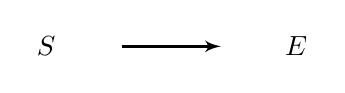
\begin{tikzpicture}[>=latex',line join=bevel,]
\pgfsetlinewidth{1bp}
\pgfsetcolor{black}

% Edge: S -> E
\draw [->] (54.403bp,18bp) .. controls (62.393bp,18bp) and (71.311bp,18bp)  .. (89.919bp,18bp);

% Node: S
\begin{scope}
  \definecolor{strokecol}{rgb}{0.0,0.0,0.0};
  \pgfsetstrokecolor{strokecol}
  \draw (27bp,18bp) node {$S$};
\end{scope}

% Node: E
\begin{scope}
  \definecolor{strokecol}{rgb}{0.0,0.0,0.0};
  \pgfsetstrokecolor{strokecol}
  \draw (117bp,18bp) node {$E$};
\end{scope}

\end{tikzpicture}

\caption[]{A  control flow graph for the empty \D{} program.}

\label{figure:cfg-empty}

\end{figure}



\subsection{Function clauses}

While node construction and destruction are primitive operations in \D{}, we'll
refrain ourselves from delving into such details in the control flow graphs of
our programs. Indeed because \emph{node construction and destruction always
terminates}. Instead, we'll let a \emph{function clause} define a point in a
program.

The expression of the clause can thereafter make calls to its
enclosing\footnote{We say that a function \emph{consists} of function clauses
and a function clause is \emph{enclosed} in a function.}, or some other
function. Such calls are represented by transfer of control, that is, arcs.
Disregarding the cases where a function clause expression makes multiple calls
to the same function with different arguments, these arcs need not be
disjunctively labelled since all of these transitions happen unconditionally as
a result of evaluating the expression. More specifically, \emph{we consider the
order of evaluation to be insignificant}, and hence undeserving of labelling.
We further discuss the reasons for this below.

If calls are separated by node construction, the order in which those calls are
made is definitely insignificant. For instance, consider the expression
\mono{(f a).(g b)}, where \mono{f} and \mono{g} are some well-defined
functions, $\text{\mono{f}}\neq\text{\mono{g}}$, and \mono{a} and \mono{b} are
some bound variables. It makes no difference to the final result which of the
calls, \mono{f a} and \mono{g b}, is evaluated first. Indeed, they can be
evaluated in parallel, and we would still get the same result. This is easy to
see for any nested construction of results of function calls, as in e.g.
\mono{(f a).0.(g b)}.

On the other hand, the syntax and semantics of \D{} allow for function calls to
be nested as in e.g. the expression \mono{(f (g a) (h b))}, where \mono{h} is
also some well-defined function and is pairwise unequal to \mono{f} and
\mono{g}. While the order of evaluation of \mono{g a} and \mono{h b} is
\emph{insignificant} wrt. to one another, as with function calls separated by
construction, the order of evaluation of these two subexpressions wrt. to the
call to function \mono{f}, \emph{is significant to the result}, and
\emph{might} be significant to termination analysis in general. However, we'll
regard this as insignificant for the time being for mere simplicity. We'll come
back to the question of whether size-change termination analysis can benefit
from regarding this as significant later on.

We can now draw a control flow graph for the program define in
\referToListing{cfg-sample-1} as shown in \referToFigure{cfg-sample-1}.

\begin{lstlisting}[label=listing:cfg-sample-1,caption={A sample \D{} program, always returning \mono{0.0.0}.}]
f x y := x.y
g _ := 0
h _ := 0
i x y := (f ((h y).(g x)) (h y))
i input input
\end{lstlisting}

\begin{figure}[htbp!]
\centering
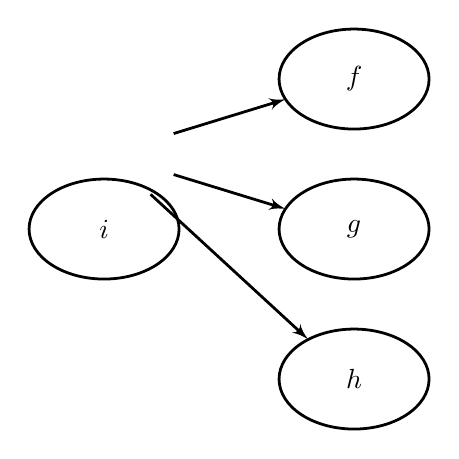
\begin{tikzpicture}[>=latex',line join=bevel,]
\pgfsetlinewidth{1bp}
\pgfsetcolor{black}

% Edge: i -> h
\draw [->] (133.73bp,84.519bp) .. controls (147.37bp,71.964bp) and (167.3bp,53.624bp)  .. (190.4bp,32.356bp);

% Edge: i -> f
\draw [->] (142.05bp,106.38bp) .. controls (151.44bp,109.26bp) and (162.36bp,112.61bp)  .. (182.29bp,118.72bp);

% Edge: i -> g
\draw [->] (142.05bp,91.622bp) .. controls (151.44bp,88.741bp) and (162.36bp,85.389bp)  .. (182.29bp,79.275bp);

% Node: g
\begin{scope}
  \definecolor{strokecol}{rgb}{0.0,0.0,0.0};
  \pgfsetstrokecolor{strokecol}
  \draw (207bp,72bp) ellipse (27bp and 18bp);
  \draw (207bp,72bp) node {$g$};
\end{scope}

% Node: f
\begin{scope}
  \definecolor{strokecol}{rgb}{0.0,0.0,0.0};
  \pgfsetstrokecolor{strokecol}
  \draw (207bp,126bp) ellipse (27bp and 18bp);
  \draw (207bp,126bp) node {$f$};
\end{scope}

% Node: i
\begin{scope}
  \definecolor{strokecol}{rgb}{0.0,0.0,0.0};
  \pgfsetstrokecolor{strokecol}
  \draw (117bp,72bp) ellipse (27bp and 18bp);
  \draw (117bp,72bp) node {$i$};
\end{scope}

% Node: h
\begin{scope}
  \definecolor{strokecol}{rgb}{0.0,0.0,0.0};
  \pgfsetstrokecolor{strokecol}
  \draw (207bp,18bp) ellipse (27bp and 18bp);
  \draw (207bp,18bp) node {$h$};
\end{scope}

\end{tikzpicture}

\caption[]{A  control flow graph for the \D{} program in
\referToListing{cfg-sample-1}. The graph does not explicitly specify
back-propagation of control, if any.}

\label{figure:cfg-sample-1}

\end{figure}



\subsection{Call cycles}

A call cycle occurs when there is a cyclical transition of control between the
nodes of a control flow graph. I.e. when there is a cycle in the control flow
graph.

\begin{lemma} We're concerned with call cycles in control flow graphs since
non-termination cannot occur if not for an infinite control flow cycle.
\end{lemma}

\begin{proof} If a program has a control flow graph with no cycles and does not
terminate, then one of the primitive operations, i.e. construction,
destruction, comparison or binding, does not terminate, which is certainly
absurd given the semantics of \D{}. \end{proof}

Call cycles in \D{} can occur in recursive or mutually recursive function
clauses.

We will henceforth refer to function clauses with recursive calls as
\emph{recursive clauses} and their counterparts, i.e. the base clauses of a
function declaration, \emph{terminal clauses}.

\subsection{Disregarding back-propagation}

It is worth noting that in \referToFigure{cfg-sample-1}, the clauses that make
no function calls have out-degree $0$. Technically, these functions \emph{do
transfer control} -- back to the callee. We may refer to this process as
\emph{back-propagation of control}. While considering back-propagation is
seemingly important to a concept that bases itself on the changes in the sizes
of the program values, we're only concerned with call cycles.

The thing with back-propagation is that forward-propagation after
back-propagation of a call cannot occur due to the way \D{} is defined. Hence,
what we are really concerned with is, ``how deep the rabbit hole goes'', before
we back-propagate, as back-propagation superimplies termination of the function
we're back-propagating out of.

\subsection{Dropping the start and end nodes}

The disregard of the back-propagation of control forces us to either redefine
the transition from the start node and the transitions to the end node. This is
because neither of these transitions are ever back-propagated, while all other
transitions \emph{must be} back-propagated if the program terminates.

Alternatively, disregard of back-propagation allows us to drop these nodes
completely and concentrate on the clauses and explicit calls within the clause
expressions. Hence, start and end nodes will not appear in any further graphs.

\subsection{Control flow graphs vs. abstract static call graphs}

Disregard of back-propagation allows us to consider control flow graphs
presented in this text as mere \emph{abstract static call graphs}, henceforth
referred to simply as, \emph{call graphs}. The abstraction applied to these
graphs compared to regular static call graphs is that the concrete arguments of
the function calls are not considered, and we merely consider how these values
can change in size from for a given function call. Interestingly, the problem
of termination analysis can be rephrased as the problem of determining whether
the regular static call graph of a program, i.e. the one containing the
concrete function arguments, is finite.

\subsection{Multiple calls to the same function}

Up until now we've only regarded expressions that don't make calls to the same
function with varying arguments. This is because these calls have to be
disjunctively labelled for the purposes of our analysis, because the use of
varying arguments \emph{may} mean varying decrease (or increase), in values for
the different calls within the expression. For this purpose we'll disjunctively
label \emph{all} the calls within an expression, if necessary, but remember
that this has nothing to do with evaluation order as has been discussed above.

This allows us to draw a control flow graph, or equivalently, a call graph,
for the program in \referToListing{cfg-sample-2}. Here, we've already
disjunctively labelled all of the calls in the expressions. This call graph is
drawn in \referToFigure{cfg-sample-2}.

\begin{lstlisting}[label=listing:cfg-sample-2,caption={A sample \D{} program, always returning \mono{(0.x).(0.y)}, where \mono{x} and \mono{y} are arbitrary \D{} values supplied by the user.}]
f x y := x.y
g x := 0.x
i x y := (0: f (1: g x) (2: g y))
i input input
\end{lstlisting}

\begin{figure}[htbp!]
\centering
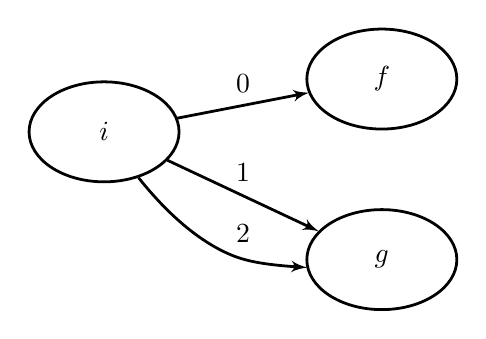
\begin{tikzpicture}[>=latex',line join=bevel,]
\pgfsetlinewidth{1bp}
\pgfsetcolor{black}

% Edge: i -> g
\draw [->] (141.75bp,53.791bp) .. controls (155.07bp,47.538bp) and (172.33bp,39.435bp)  .. (196.31bp,28.18bp);

\definecolor{strokecol}{rgb}{0.0,0.0,0.0};
\pgfsetstrokecolor{strokecol}
\draw (169bp,49.5bp) node {$1$};

% Edge: i -> g
\draw [->] (131.41bp,47.488bp) .. controls (139.3bp,37.571bp) and (150.73bp,25.786bp)  .. (164bp,20bp) .. controls (169.56bp,17.574bp) and (175.77bp,16.246bp)  .. (192.14bp,15.146bp);
\draw (169bp,27.5bp) node {$2$};

% Edge: i -> f
\draw [->] (145.24bp,68.893bp) .. controls (156.67bp,71.109bp) and (170.38bp,73.767bp)  .. (192.85bp,78.124bp);
\draw (169bp,81.5bp) node {$0$};

% Node: i
\begin{scope}
  \definecolor{strokecol}{rgb}{0.0,0.0,0.0};
  \pgfsetstrokecolor{strokecol}
  \draw (119bp,64bp) ellipse (27bp and 18bp);
  \draw (119bp,64bp) node {$i$};
\end{scope}

% Node: g
\begin{scope}
  \definecolor{strokecol}{rgb}{0.0,0.0,0.0};
  \pgfsetstrokecolor{strokecol}
  \draw (219bp,18bp) ellipse (27bp and 18bp);
  \draw (219bp,18bp) node {$g$};
\end{scope}

% Node: f
\begin{scope}
  \definecolor{strokecol}{rgb}{0.0,0.0,0.0};
  \pgfsetstrokecolor{strokecol}
  \draw (219bp,83bp) ellipse (27bp and 18bp);
  \draw (219bp,83bp) node {$f$};
\end{scope}
%
\end{tikzpicture}

\caption[]{A  control flow graph for the \D{} program in \referToListing{cfg-sample-2}.}

\label{figure:cfg-sample-2}

\end{figure}



\subsection{Multiple clauses}

If function clauses are nodes, and the function calls within the expressions of
the function clauses are unconditional transitions, what exactly happens if the
arguments supplied to the function clause fail to match the pattern declaration
for the clause?

The semantics of \D{} tell us to make an unconditional transition to the
immediately next clause of the function. There is at most one such transition
for any clause, and the last clause of a function declaration cannot fail to
pattern match\footnote{See \referToSection{d-sos}.}.

We'll refer to these transitions as \emph{fail transitions} and visually mark
them with a dotted line rather than a filled line. We need this way of visually
distinguishing fail transitions from the rest since they are conditionally
different, in that for any clause with a fail transition, either the fail
transition is chosen, or all the non-fail transitions are chosen
simultaneously.

Before we can draw the call graph we also need a way to distinguish the clauses
of a function wrt. the program text. We decide to enumerate the clauses
top-to-bottom starting with 0. Sometimes we'll annotate the program text with
these unique labels for each clause to make the call graph more readable.

Hence, we can now draw the call graph for the program defined in
\referToListing{cfg-loop} as shown in \referToFigure{cfg-loop}.

\begin{lstlisting}[label=listing:cfg-loop,caption={A simple, down-counting loop in \D{}.}]
f0: f 0 := 0
f1: f x._ := f x

f input
\end{lstlisting}

\begin{figure}[htbp!]
\centering
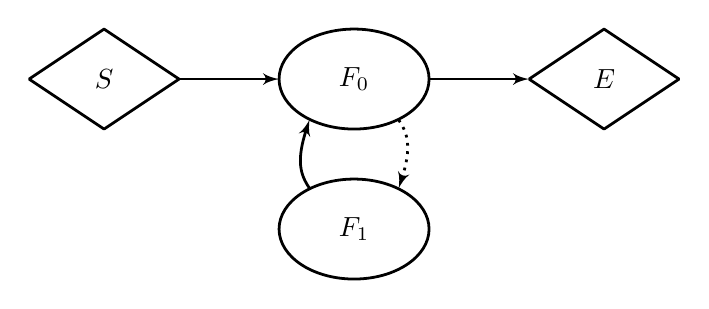
\begin{tikzpicture}[>=latex',line join=bevel,]

\pgfsetlinewidth{1bp}
\pgfsetcolor{black}

% Edge: F0 -> F1
\draw [->,dotted] (133.06bp,73.287bp) .. controls (136.46bp,68.306bp) and (137.79bp,63.325bp)  .. (133.09bp,48.766bp);

% Edge: S -> F0
\draw [->] (54.403bp,88bp) .. controls (62.393bp,88bp) and (71.311bp,88bp)  .. (89.919bp,88bp);

% Edge: F1 -> F0
\draw [->] (100.91bp,48.766bp) .. controls (97.522bp,53.747bp) and (96.204bp,58.727bp)  .. (100.94bp,73.287bp);

% Edge: F0 -> E
\draw [->] (144.4bp,88bp) .. controls (152.39bp,88bp) and (161.31bp,88bp)  .. (179.92bp,88bp);

% Node: F0
\begin{scope}
  \definecolor{strokecol}{rgb}{0.0,0.0,0.0};
  \pgfsetstrokecolor{strokecol}
  \draw (117bp,88bp) ellipse (27bp and 18bp);
  \draw (117bp,88bp) node {$F_0$};
\end{scope}

% Node: F1
\begin{scope}
  \definecolor{strokecol}{rgb}{0.0,0.0,0.0};
  \pgfsetstrokecolor{strokecol}
  \draw (117bp,34bp) ellipse (27bp and 18bp);
  \draw (117bp,34bp) node {$F_1$};
\end{scope}

% Node: S
\begin{scope}
  \definecolor{strokecol}{rgb}{0.0,0.0,0.0};
  \pgfsetstrokecolor{strokecol}
  \draw (27bp,106bp) -- (0bp,88bp) -- (27bp,70bp) -- (54bp,88bp) -- cycle;
  \draw (27bp,88bp) node {$S$};
\end{scope}

% Node: E
\begin{scope}
  \definecolor{strokecol}{rgb}{0.0,0.0,0.0};
  \pgfsetstrokecolor{strokecol}
  \draw (207bp,106bp) -- (180bp,88bp) -- (207bp,70bp) -- (234bp,88bp) -- cycle;
  \draw (207bp,88bp) node {$E$};
\end{scope}

\end{tikzpicture}

\caption[]{A  control flow graph for the program defined in
\referToListing{d-loop}.}

\label{figure:cfg-loop}

\end{figure}

 

For a more complex example, let's consider the call graph for the program
\mono{reverse} introduced in \referToSection{d-samples}. The program is
repeated in annotated form in \referToListing{cfg-reverse}, and its
corresponding call graph is shown in \referToFigure{cfg-reverse}.

\begin{lstlisting}[label=listing:cfg-reverse,caption={An annotated version of the program \mono{reverse} introduced in \referToSection{d-samples}.}]
r0: reverse 0 := 0
r1: reverse left.right := (0: reverse right).(1: reverse left)

reverse input
\end{lstlisting}

\begin{figure}[htbp!]
\centering
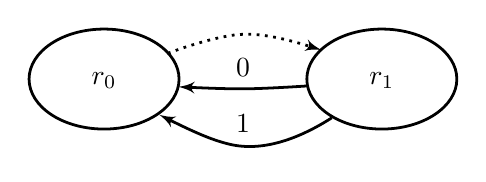
\begin{tikzpicture}[>=latex',line join=bevel,]
\pgfsetlinewidth{1bp}
\pgfsetcolor{black}

% Edge: R0 -> R1
\draw [->,dotted] (49.969bp,34.268bp) .. controls (56.882bp,36.851bp) and (64.635bp,39.282bp)  .. (72bp,40.58bp) .. controls (79.767bp,41.948bp) and (88bp,40.866bp)  .. (105.24bp,35.467bp);

% Edge: R1 -> R0
\draw [->] (99.957bp,22.51bp) .. controls (94.056bp,22.123bp) and (87.816bp,21.778bp)  .. (82bp,21.58bp) .. controls (76.252bp,21.384bp) and (70.164bp,21.454bp)  .. (53.809bp,22.204bp);

\definecolor{strokecol}{rgb}{0.0,0.0,0.0};
\pgfsetstrokecolor{strokecol}
\draw (77bp,29.08bp) node {$0$};

% Edge: R1 -> R0
\draw [->] (108.98bp,11.053bp) .. controls (98.589bp,4.4007bp) and (84.865bp,-1.5798bp)  .. (72bp,1.5798bp) .. controls (66.559bp,2.9161bp) and (61.044bp,5.0566bp)  .. (46.908bp,12.145bp);
\draw (77bp,9.0798bp) node {$1$};

% Node: R0
\begin{scope}
  \definecolor{strokecol}{rgb}{0.0,0.0,0.0};
  \pgfsetstrokecolor{strokecol}
  \draw (27bp,25bp) ellipse (27bp and 18bp);
  \draw (27bp,24.58bp) node {$r_0$};
\end{scope}

% Node: R1
\begin{scope}
  \definecolor{strokecol}{rgb}{0.0,0.0,0.0};
  \pgfsetstrokecolor{strokecol}
  \draw (127bp,25bp) ellipse (27bp and 18bp);
  \draw (127bp,24.58bp) node {$r_1$};
\end{scope}
%
\end{tikzpicture}

\caption[]{A  control flow graph for the \D{} program in \referToListing{cfg-reverse}.}

\label{figure:cfg-reverse}

\end{figure}
 

\subsection{Deeply nested function calls}

Blah

\section{Size-change termination principle}

Consider the program in \referToListing{cfg-loop} and it's corresponding call
graph in \referToFigure{cfg-loop}. Without any further information about the
control transitions, the program seemingly loops indefinitely. However, there
are some things that we can deduce about the control transitions.

\begin{lemma} If we can deduce for every control flow cycle in a prorgram that
it reduces a value of well-founded data-type on each iteration of the cycle,
then the value must eventually bottom out and the program must terminate.
\end{lemma}

\begin{proof} Assume for the sake of contradiction that a program that reduces
a value of a well-founded data type in each call cycle does not terminate.
Then, either the value reduces indefinitely, which is a contradiction to the
well-foundedness of its data type, or some noncyclic call sequence causes an
infinite loop, also an absurdity due to the definition of \D{}. \end{proof}

That is the \emph{size-change termination principle}. All values in \D{} are
inherently well-founded so what remains to be shown is how we can deduce from a
call cycle whether it reduces a value on each iteration.

\begin{lemma}\label{lemma:cycle-reduce} A control flow cycle reduces a value on
each iteration if at least one of the participating control transitions reduces
the value and all other control transitions do not increase that
value.\end{lemma}

\begin{proof} If a value is not reduced in a cycle, it either stays the same or
is increased. If it is increased, then at least one control transition must've
increased the value, an absurdity. If it stays the same then none of the
participating control transitions have neither increased nor decreased the
value, also an absurdity. \end{proof}

By the definition of call graphs, function clauses participate as nodes in a
call cycle. A control transition is a directed edge between two function
clauses where one clause is the \emph{source} and the other is the
\emph{target}. 

We can analyze how a value changes it's size through a call sequence by
analyzing the size relation between the variables bound in the source and the
variables bound in the target of every control transition.

\begin{definition} The relation $\Phi\ :\ C_{caller} \times C_{callee} \times
N_{caller} \times N_{callee} \rightarrow \{\bot,<,\leq\}$ is defined to be the
size relation between the caller and callee
clauses in \D{} where $N_{caller}$ are the names of the variables bound in the
caller, and $N_{callee}$ are the names of the variables bound in the callee.
Note, that we are only concerned with reductions and non-increases in size, all
other relationships are marked by the no relationship symbol $\bot$. Initially,
the relationship between all the clauses and their variables is $\bot$.
\end{definition}

The construction of the relationship $\Phi$ for a given transition depends
first and foremost on whether that transition is a fail or success transition.

\subsection{Fail transitions}

A fail transition occurs if the values passed to a given clause to match it's
pattern. If the values fail to match the pattern, no variables are bound and
hence no change in values can occur. The values are simply passed along as they
were to the next clause of the function declaration.

\begin{lemma} Fail transitions are transitive in the sense that the
relationship between the variables bound in the source and the variables bound
in the target is the same regardless of the number of fail transitions in
the path between the source and the target.\end{lemma}

\begin{proof} Follows from the semantics of \D{}. \end{proof}

We are not concerned with exact equivalence, hence all fail transitions in the
$\Phi$ relation return the relation $\leq$ for all variable pairs.

Note, that due to \D{} being first order and statically scoped, the variable
space is always initially empty when a function clause begins pattern matching.

\subsection{Success transitions}

Since \D{} is a call-by-value language, when a function call is encountered,
the source evaluates the arguments of the function call and generates some
\emph{values} before giving up control.

The values may hence be a nested construction of some concrete values, values
bound to variables in the source, and results of nested function calls. Without
further regard of nested function calls, this implies that a \emph{size
relation} can be deduced between the variables bound in the source and the
values that result from an evaluation of the function call arguments. 

Of course, we cannot deduce a precise size displacement as the values of the
bound variables may initially be \emph{unknown} at compile
time\footnote{Although some values can be deduced via static analysis of the
program, others can come in from the outside world via the 0-ary function
\mono{input} at run time.}.  However, we can deduce a \emph{safe} displacement
estimate, such that it is less than or equal to the actual displacement in
terms of absolute value. For instance, if the expression \mono{a.b} appears as
a function call argument, where \mono{a} and \mono{b} are some bound variables
with unknown values, and this argument evaluates to some value $v$, then we can
\emph{safely} say that $v>\text{\mono{a}}$, $v>\text{\mono{b}}$,
$v\geq\text{\mono{a.0}}$ and $v\geq\text{\mono{0.b}}$.

We decide to ignore the nested function calls because this would imply a more
complex static analysis of the program. Specifically, we're unable to say
anything about the result of the nested function call from the scope of the
source clause alone. Instead, we treat results from nested function calls
simply as variables with \emph{unknown} values. We also make sure to keep these
variables separate from the bound variables as there is no relationship to draw
between these ``variables'' and the variables bound in the
target\footnote{While this information may be useful for dead-code elimination
and other forms of static analysis, this is of little importance to size-change
termination.}.

More formally, given a function argument as the expression $x$, we construct
the expression $x^s$ where we replace all first-level nested function
calls\footnote{Nested function calls of nested function calls are hence
considered irrelevant to the derivation of the size relation of the top-level
call, however, they may become relevant as we derive the size relations of the
corresponding nested calls.} by auxiliary variables.  We group all those
auxiliary variables into the set of variable names $N_{calls}^s$ and all the
remaining variables into the set $N_{vars}^s$.  Furthermore we construct the
auxiliary variable names in such way that $N_{vars}^s\cup
N_{calls}^s=\emptyset$.  Hence, we obtain the tuple
$(x^c,N_{vars}^s,N_{calls}^s)$.

Continuing on with the example above, i.e. having the size relations
$\{v>\textt{a}, v> \textt{b}, v\geq \textt{a.0}, v\geq \textt{0.b}\}$, assume
that the target clause has the corresponding pattern \mono{x.y}. The question
henceforth is how do we draw the relationship that $\textt{a}\equiv\textt{x}$
and $\textt{b}\equiv\textt{y}$, or perhaps simply that the control transition
neither decreases nor increases any values. We can perform a corresponding
analysis on the pattern declaration and deduce the set of conditions that will
hold after pattern matching succeeds, indeed, $\{v>\textt{x}, v> \textt{y},
v\geq \textt{x.0}, v\geq \textt{0.y}\}$. The participation of $x$ in the same
kind of relations as $a$, and the participation of $y$ in the same kind of
relations as $b$, does not alone indicate their respective equivalence, since
the actual property that $v\equiv\textt{a.b}$ is lost.

On the other hand, if we had to formally define the relation that had to be
built between the variables bound in the source and the values that the
function call arguments evaluated to, this would be a relation between values
and some kind of ``abstract patterns'', as e.g. $v\geq\textt{0.b}$.

To simplify the entire process, instead of deducing actual size relations
between the variables bound in the source and the values that the function
arguments evaluate to, we can simply turn the function argument into the
abstract pattern to begin with. The actual size relations are hence withkept
and can be deduced at a later stage in the process.

Indeed, the tuple $(x^s,N_{vars}^s,N_{calls}^s)$ constitutes such an abstract
pattern already, since the expression $x^s$, contains no function calls and
hence syntactically matches a pattern in \D{}\footnote{See
\referToSection{d-syntax} if you're uncertain.}. We henceforth refer to such an
expression as $p^s$\footnote{Where $s$ stands for \emph{source}.}. Given a
clause with the pattern $p^t$\footnote{Where $t$ stands for \emph{target}.}, we
can easily deduce the set $N_{vars}^t$, which is the set of variable names used
in $p$. Our task is then to deduce a size relation between the variables in the
sets $N_{vars}^s$ and $N_{vars}^t$ given the tuples
$(p^s,N_{vars}^s,N_{calls}^s)$ and $(p^t,N_{vars}^t)$.

\subsection{Pattern matching}

Let the function $\phi\ :\ \mathbb{N} \times \mathbb{N} \rightarrow
\{<,\leq,\bot\}$ denote the function $\lambda N^t, N^s .
\Phi\left(C^t,C^s,N^t,N^s\right)$. In the following section we will discuss the
rules involved in deducing the function $\phi$, that is, the function $\Phi$
for some given source and target of a success transition.

For this purpose we will regard the tuples $(P^s,N_{vars}^s)$ and
$(P^t,N_{vars}^t)$, of a given success transition, where $P^s$ is the list of
abstract patterns derived from the function arguments in the source, and $P^t$
is the list of corresponding actual patterns in the target. Furthermore, let
$N_{vars}^s$ and $N_{vars}^t$ be unary functions of the type
$\mathbb{P}\rightarrow\mathbb{N}^*$, accepting a pattern and yielding the
variable names that are contained both in the input pattern and the sets
$N_{vars}^s$ and $N_{vars}^t$, respectively.

In the following analysis we will look at but one instance of the lists $P^s$
and $P^t$, namely the abstract pattern $p^s$ from the source and its
corresponding actual pattern in the declaration, $p^t$. In total, however, this
process has to be repeated for each such pair given the sets $P^s$ and $P^t$,
iteratively extending the definition of the relation $\phi$ to all variables
bound in the sets $N_{vars}^s$ and $N_{vars}^t$.

We initially define $\phi$ to yield the value $\bot$ for all arguments. We will
continuously modify this definition as we process $p^s$ and $p^t$. We denote
this within the semantics in a manner similar to the state $\sigma$ in the
semantics\footnote{See \referToSection{d-sos}.}. However, $\phi$ is now a
binary ``memory'', requiring both a target name and a source name (in that
order). For simplicity, we will borrow some suger coding from the matlab
notation which allows us to provide a collection in place of a single element
and let the runtime apply the given function to each element in the collection.
For instance, we might write that $\phi\left(N_{vars}^t(p^t), n^s\right)\mapsto
<$, meaning that all the target variables used in $p^t$ are strictly less than
the source variable $n^s$.

We now define a summoning rule, dividing the rules up into sub-rules:

\begin{equation}
{
    \left\langle\proc{A},p^t,p^s,\phi\right\rangle
    \rightarrow
    \phi'
  \vee
    \left\langle\proc{B},p^t,p^s,\phi\right\rangle
    \rightarrow
    \phi'
  \vee
    \left\langle\proc{C},p^t,p^s,\phi\right\rangle
    \rightarrow
    \phi'
  \vee
    \left\langle\proc{D},p^t,p^s,\phi\right\rangle
    \rightarrow
    \phi'
  \vee
    \left\langle\proc{E},p^t,p^s,\phi\right\rangle
    \rightarrow
    \phi'
}\over{
  \left\langle p^t,p^s,\phi\right\rangle
  \rightarrow
  \phi'
}
\end{equation}

One of the simpler cases is when the abstract pattern $p^s$ is simply \mono{0},
or some name $n^s$, and $n^s\in N_{calls}^s$. Since no variables bound in the
source participate in $p^s$, then no relations need to be drawn to any of the
target variables that might appear in the corresponding $p^t$. Hence, $\phi$
need not be modified.

\begin{equation}\label{eq:sct-pattern-source-fail}
{
\left(
    p^s\rightarrow 0
  \vee
\left(
    p^s\rightarrow n^s
  \wedge
    n^s\notin N_{vars}^s
\right)
\right)
  \wedge
    \phi\rightarrow\phi'
}\over{
  \left\langle\proc{A},p^t,p^s,\phi\right\rangle
  \rightarrow
  \phi'
}
\end{equation}

This has a symmetrical case. Indeed when $p^t$ is neither a destruction, nor
any name $n^t$, that is, it is \mono{\_} or \mono{0}. This pattern contains no
variables, and hence  no relations need to be drawn from any of the variables
that might appear in the corresponding $p^s$. Hence, $\phi$ need not be
modified in such a case either.

\begin{equation}
{
\left(
    p^t\rightarrow 0
\vee
    p^t\rightarrow \_
\right)
  \wedge
    \phi\rightarrow\phi'
}\over{
  \left\langle\proc{B},p^t,p^s,\phi\right\rangle
  \rightarrow
  \phi'
}
\end{equation}

If $p^t$ is the name pattern $n^t$, the matters get a bit more complicated:

\begin{enumerate}

\item If $p^s$ is some node, then all the variables that occur in $p^s$, i.e.
$N_{vars}^s(p^s)$, will all be strictly less than $n^t$ by the semantics of
\D{}. However, we are not concerned with this relation, as we would like to
know when a value is decreased from source to target, and not, as in this case,
increased.

\item If $p^s$ is also some name pattern $n^s$, and  $n^s\in N^s_{vars}$, then
the values of these corresponding variables will be \emph{equivalent}. However,
we're not concerned with exact equivalence, and simply mark this relationship
with the weaker, but still sound relation, $\leq$:

\begin{equation}
{
    p^t\rightarrow n^t
  \wedge
    p^s\rightarrow n^s
  \wedge
    n^s\in N_{vars}^s
  \wedge
    \left\langle\phi\left(n^t, n^s\right)\mapsto \leq\right\rangle\rightarrow\phi'
}\over{
  \left\langle\proc{C},p^t,p^s,\phi\right\rangle
  \rightarrow
  \phi'
}
\end{equation}

\end{enumerate}

If $p^t$ is a destruction and $p^s$ is the variable name $n^s$, then we can safely say that
all the variables that occur in $p^t$, i.e. $N_{vars}^t(p^t)$, are all strictly less
than the variable in $n^s$:

\begin{equation}
{
    p^t\rightarrow p^t_1\cdot p^t_2
  \wedge
    p^s\rightarrow n^s
  \wedge
    n^s\in N_{vars}^s
  \wedge
    \left\langle\phi\left(N_{vars}^t(p^t), n^s\right)\mapsto <\right\rangle\rightarrow\phi'
}\over{
  \left\langle\proc{D},p^t,p^s,\phi\right\rangle
  \rightarrow
  \phi'
}
\end{equation}

If both $p^t$ and $p^s$ are a destructions, then the following recursive rule applies:

\begin{equation}
{
    p^t\rightarrow p^t_1\cdot p^t_2
  \wedge
    p^s\rightarrow p^s_1\cdot p^s_2
  \wedge
    \left\langle p^t_1, p^s_1, \phi\right\rangle
    \rightarrow
    \phi''
  \wedge
    \left\langle p^t_2, p^s_2, \phi''\right\rangle
    \rightarrow
    \phi'
}\over{
  \left\langle\proc{E},p^t,p^s,\phi\right\rangle
  \rightarrow
  \phi'
}
\end{equation}

\section{Graph annotation}

Hence, we can deduce from \referToListing{cfg-loop}, that when $f_1$ makes a
call to $f_0$ it does so with a value strictly less then it's own argument,
i.e. the transition $f_1\rightarrow f_0$ strictly decreases a value. Visually
we will mark this with a $\downarrow$. The Lemmas \refer{lemma:d-pattern-leq}
and \refer{lemma:d-pattern-less} can be used to deduce the same sort of
relationship for the transitions $r_1\xrightarrow{0,1} r_0$ for
\referToListing{cfg-reverse}. These observations are summarised in
\referToFigure{sct-first}.

\begin{figure}[htbp!]
\centering

\subfigure[The program in \referToListing{cfg-loop}.]{
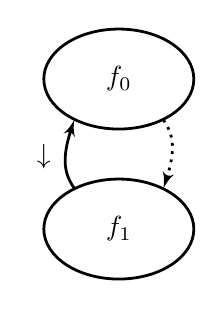
\begin{tikzpicture}[>=latex',line join=bevel,]

\pgfsetlinewidth{1bp}
\pgfsetcolor{black}

% Edge: F0 -> F1
\draw [->,dotted] (133.06bp,73.287bp) .. controls (136.46bp,68.306bp) and (137.79bp,63.325bp)  .. (133.09bp,48.766bp);

\draw (90bp,60bp) node {$\downarrow$};

% Edge: F1 -> F0
\draw [->] (100.91bp,48.766bp) .. controls (97.522bp,53.747bp) and (96.204bp,58.727bp)  .. (100.94bp,73.287bp);

% Node: F0
\begin{scope}
  \definecolor{strokecol}{rgb}{0.0,0.0,0.0};
  \pgfsetstrokecolor{strokecol}
  \draw (117bp,88bp) ellipse (27bp and 18bp);
  \draw (117bp,88bp) node {$f_0$};
\end{scope}

% Node: F1
\begin{scope}
  \definecolor{strokecol}{rgb}{0.0,0.0,0.0};
  \pgfsetstrokecolor{strokecol}
  \draw (117bp,34bp) ellipse (27bp and 18bp);
  \draw (117bp,34bp) node {$f_1$};
\end{scope}

\end{tikzpicture}
}

\subfigure[The program in \referToListing{cfg-reverse}.]{
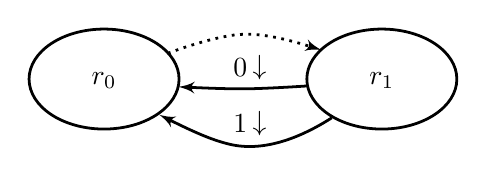
\begin{tikzpicture}[>=latex',line join=bevel,]
\pgfsetlinewidth{1bp}
\pgfsetcolor{black}

% Edge: R0 -> R1
\draw [->,dotted] (49.969bp,34.268bp) .. controls (56.882bp,36.851bp) and (64.635bp,39.282bp)  .. (72bp,40.58bp) .. controls (79.767bp,41.948bp) and (88bp,40.866bp)  .. (105.24bp,35.467bp);

% Edge: R1 -> R0
\draw [->] (99.957bp,22.51bp) .. controls (94.056bp,22.123bp) and (87.816bp,21.778bp)  .. (82bp,21.58bp) .. controls (76.252bp,21.384bp) and (70.164bp,21.454bp)  .. (53.809bp,22.204bp);

\definecolor{strokecol}{rgb}{0.0,0.0,0.0};
\pgfsetstrokecolor{strokecol}

\draw (76bp,29.08bp) node {$0$};
\draw (83bp,29.08bp) node {$\downarrow$};

% Edge: R1 -> R0
\draw [->] (108.98bp,11.053bp) .. controls (98.589bp,4.4007bp) and (84.865bp,-1.5798bp)  .. (72bp,1.5798bp) .. controls (66.559bp,2.9161bp) and (61.044bp,5.0566bp)  .. (46.908bp,12.145bp);

\draw (76bp,9.0798bp) node {$1$};
\draw (83bp,9.0798bp) node {$\downarrow$};

% Node: R0
\begin{scope}
  \definecolor{strokecol}{rgb}{0.0,0.0,0.0};
  \pgfsetstrokecolor{strokecol}
  \draw (27bp,25bp) ellipse (27bp and 18bp);
  \draw (27bp,24.58bp) node {$r_0$};
\end{scope}

% Node: R1
\begin{scope}
  \definecolor{strokecol}{rgb}{0.0,0.0,0.0};
  \pgfsetstrokecolor{strokecol}
  \draw (127bp,25bp) ellipse (27bp and 18bp);
  \draw (127bp,24.58bp) node {$r_1$};
\end{scope}
%
\end{tikzpicture}
}

\caption[]{Call graphs with annotated edges for various programs.}

\label{figure:sct-first}

\end{figure}


\subsection{Calls to multivariate functions}

The call graph notation used thus far has only been used for describing calls
to unary functions. As an example of a multivariate function, we may consider
the function \mono{normalized-less/2}, introduced in
\referToSection{d-size-less}. We use this function to define the program in
\referToListing{sct-normalized-less}. The corresponding call graph is shown in
\referToFigure{sct-normalized-less}.

\begin{lstlisting}[
  label={listing:sct-normalized-less},
  caption={A sample program with a multivariate function.}]
n0: normalized-less 0 b := b
n1: normalized-less _ 0 := 0
n2: normalized-less _.a _.b := normalized-less a b
normalized-less input input
\end{lstlisting}

\begin{figure}[htbp!]
\centering
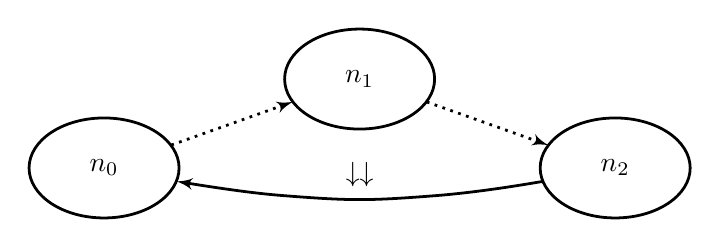
\begin{tikzpicture}[>=latex',line join=bevel,]
\pgfsetlinewidth{1bp}
\pgfsetcolor{black}

% Edge: n0 -> n1
\draw [->,dotted] (51.177bp,26.241bp) .. controls (61.57bp,29.936bp) and (74.012bp,34.36bp)  .. (94.901bp,41.787bp);

% Edge: n1 -> n2
\draw [->,dotted] (143.18bp,41.759bp) .. controls (153.57bp,38.064bp) and (166.01bp,33.64bp)  .. (186.9bp,26.213bp);

% Edge: n2 -> n0
\draw [->] (184.88bp,13.152bp) .. controls (173.12bp,11.121bp) and (158.89bp,9.0013bp)  .. (146bp,8bp) .. controls (122.07bp,6.1419bp) and (115.93bp,6.1419bp)  .. (92bp,8bp) .. controls (82.632bp,8.7275bp) and (72.561bp,10.045bp)  .. (53.124bp,13.152bp);

\definecolor{strokecol}{rgb}{0.0,0.0,0.0};
\pgfsetstrokecolor{strokecol}
\draw (119bp,15.5bp) node {$\downarrow\downarrow$};

% Node: n0
\begin{scope}
  \definecolor{strokecol}{rgb}{0.0,0.0,0.0};
  \pgfsetstrokecolor{strokecol}
  \draw (27bp,18bp) ellipse (27bp and 18bp);
  \draw (27bp,18bp) node {$n_0$};
\end{scope}

% Node: n1
\begin{scope}
  \definecolor{strokecol}{rgb}{0.0,0.0,0.0};
  \pgfsetstrokecolor{strokecol}
  \draw (119bp,50bp) ellipse (27bp and 18bp);
  \draw (119bp,50bp) node {$n_1$};
\end{scope}
% Node: n2
\begin{scope}
  \definecolor{strokecol}{rgb}{0.0,0.0,0.0};
  \pgfsetstrokecolor{strokecol}
  \draw (211bp,18bp) ellipse (27bp and 18bp);
  \draw (211bp,18bp) node {$n_2$};
\end{scope}
%
\end{tikzpicture}

\caption[]{A  control flow graph for the program defined in
\referToListing{sct-normalized-less}.}

\label{figure:sct-normalized-less}

\end{figure}



The notation is straightforward, the juxtaposition of the $\downarrow$
indicates the size change of the respective arguments, read left to right as in
the function clause definition.

\subsection{Nonincreasing transitions}

There are cases where for a given transition in a call cycle, we can't tell
whether the sizes are strictly decreased or remain the same, but we can
definitely say that there is \emph{no increase} in the sizes of variables. As
an example, consider the program in \referToListing{sct-non-reducing}.

\begin{lstlisting}[
  label=listing:sct-non-reducing,
  caption={The binary function \mono{g} has a call cycle with nonincreasing
    sizes in variables.}]
g0: g 0 0 = 0
g1: g _.a b._ = g 0.a b.0
g input input
\end{lstlisting}


For the recursive clause $g_1$, it is unclear whether the sizes of the
variables are decreased in the transition $g_1\rightarrow g_0$, or not.
Specifically, if the arguments to \mono{g} are of the form \mono{0.\_} and
\mono{\_.0}, respectively, the size is \emph{not} decreased by the call. We'll
denote such transitions by the symbol $\Downarrow$. We can now draw the call
graph for the program in \referToListing{sct-non-reducing} as in
\referToFigure{sct-non-reducing}.

\begin{figure}[htbp!]
\centering
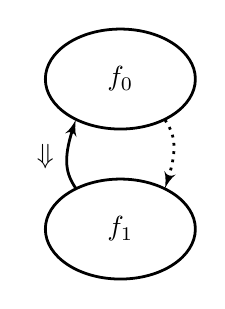
\begin{tikzpicture}[>=latex',line join=bevel,]

\pgfsetlinewidth{1bp}
\pgfsetcolor{black}

% Edge: F0 -> F1
\draw [->,dotted] (133.06bp,73.287bp) .. controls (136.46bp,68.306bp) and (137.79bp,63.325bp)  .. (133.09bp,48.766bp);

\draw (90bp,60bp) node {$\Downarrow$};

% Edge: F1 -> F0
\draw [->] (100.91bp,48.766bp) .. controls (97.522bp,53.747bp) and (96.204bp,58.727bp)  .. (100.94bp,73.287bp);

% Node: F0
\begin{scope}
  \definecolor{strokecol}{rgb}{0.0,0.0,0.0};
  \pgfsetstrokecolor{strokecol}
  \draw (117bp,88bp) ellipse (27bp and 18bp);
  \draw (117bp,88bp) node {$f_0$};
\end{scope}

% Node: F1
\begin{scope}
  \definecolor{strokecol}{rgb}{0.0,0.0,0.0};
  \pgfsetstrokecolor{strokecol}
  \draw (117bp,34bp) ellipse (27bp and 18bp);
  \draw (117bp,34bp) node {$f_1$};
\end{scope}

\end{tikzpicture}

\caption[]{An annotated call graph for the program in \referToListing{sct-non-reducing}.}

\label{figure:sct-non-reducing}

\end{figure}


\subsection{Increasing transitions}


%Values are not always decreasing.

%Consider the following program:

\begin{lstlisting}[
  label=listing:sct-infinite-join,
  caption={The function \mono{infinite-join/2} infinitely joins..}]
f0: f a b = f a.b b.a
f input input
\end{lstlisting}

%The function clause expression constructs a new value by joining the two
%incoming arguments into a new node. While we're unable to say by how much the
%values are increased exactly, we know that both values are increased by at
%least 1 due to the creation of a node for each argument.


%\newpage

%A derrivable property from the program text is that the value sent as the
%argument in the transition $F_1\rightarrow F_0$ is \emph{always} strictly less
%than the value sent as the argument in the preceeding transition,
%$F_0\rightarrow F_1$. Additionally, we can universally state that \emph{false
%transitions from case nodes by definition can't change any values}. Hence, the
%infinite control flow sequence $F_0\rightarrow F_1\rightarrow F_0$ strictly
%decreases a well founded value in every iteration of the control flow cycle.
%This means that eventually the value bottoms out at $0$ which would validate
%the $F_0$ pattern and lead the program to terminate. In general, we can state
%the following:

%\begin{lemma}

%An infinite control flow sequnece infinitely decreases a well founded value if
%all the transitions in the corresponding control flow graph cycle either
%strictly decrease a value or keep all values unchanged, and at least one
%transition strictcly decreases a value.

%\end{lemma}

%\referToFigure{cfg-loop-down} showcases an edge-labelled control flow graph for
%\referToListing{d-loop}. Transitions for which we can \emph{safely} say that a
%value is decreased we mark with the symbol $\downarrow$, transitions for which
%we can \emph{safely} say that no value is increased we mark with the symbol
%$\top$. The graph is rather verbose and in future graphs we'll omit $\top$
%labels for nodes that universally can't increase a value, i.e. $S\rightarrow
%F_0$, $F_0\rightarrow E$ and $F_0\rightarrow F_1$.

%We can further prove the soundness of the size-change termination principle.

%\begin{proof} Assume for the sake of contradiction that there exists an
%infinite control flow sequence that infinitely decreases a well-founded data
%value. Assume furthermore that the program does not terminate. Then, some
%variable has to decrease indefinately, which contradicts with the definition of
%well-founded values. \end{proof}

%Unfortunately, this particular program can be trivially unfolded into a loop
%program, so the point of using size-change termination analysis may seem
%superflous. Indeed, the only change wrt. the control flow diagram is the
%notaiton used in the diagram. For such programs, the termination property is
%easily derrivable\cite{complexity-of-loop-programs}. 


\section{Graph annotation}

Hence, we can deduce from \referToListing{cfg-loop}, that when $f_1$ makes a
call to $f_0$ it does so with a value strictly less then its own argument,
i.e. the transition $f_1\rightarrow f_0$ strictly decreases a value. Visually
we will mark this with a $\downarrow$. The Lemmas \refer{lemma:d-pattern-leq}
and \refer{lemma:d-pattern-less} can be used to deduce the same sort of
relationship for the transitions $r_1\xrightarrow{0,1} r_0$ for
\referToListing{cfg-reverse}. These observations are summarised in
\referToFigure{sct-first}.

\begin{figure}[htbp!]
\centering

\subfigure[The program in \referToListing{cfg-loop}.]{
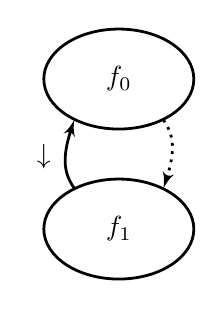
\begin{tikzpicture}[>=latex',line join=bevel,]

\pgfsetlinewidth{1bp}
\pgfsetcolor{black}

% Edge: F0 -> F1
\draw [->,dotted] (133.06bp,73.287bp) .. controls (136.46bp,68.306bp) and (137.79bp,63.325bp)  .. (133.09bp,48.766bp);

\draw (90bp,60bp) node {$\downarrow$};

% Edge: F1 -> F0
\draw [->] (100.91bp,48.766bp) .. controls (97.522bp,53.747bp) and (96.204bp,58.727bp)  .. (100.94bp,73.287bp);

% Node: F0
\begin{scope}
  \definecolor{strokecol}{rgb}{0.0,0.0,0.0};
  \pgfsetstrokecolor{strokecol}
  \draw (117bp,88bp) ellipse (27bp and 18bp);
  \draw (117bp,88bp) node {$f_0$};
\end{scope}

% Node: F1
\begin{scope}
  \definecolor{strokecol}{rgb}{0.0,0.0,0.0};
  \pgfsetstrokecolor{strokecol}
  \draw (117bp,34bp) ellipse (27bp and 18bp);
  \draw (117bp,34bp) node {$f_1$};
\end{scope}

\end{tikzpicture}
}

\subfigure[The program in \referToListing{cfg-reverse}.]{
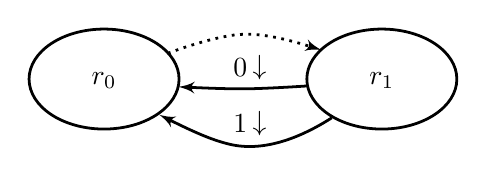
\begin{tikzpicture}[>=latex',line join=bevel,]
\pgfsetlinewidth{1bp}
\pgfsetcolor{black}

% Edge: R0 -> R1
\draw [->,dotted] (49.969bp,34.268bp) .. controls (56.882bp,36.851bp) and (64.635bp,39.282bp)  .. (72bp,40.58bp) .. controls (79.767bp,41.948bp) and (88bp,40.866bp)  .. (105.24bp,35.467bp);

% Edge: R1 -> R0
\draw [->] (99.957bp,22.51bp) .. controls (94.056bp,22.123bp) and (87.816bp,21.778bp)  .. (82bp,21.58bp) .. controls (76.252bp,21.384bp) and (70.164bp,21.454bp)  .. (53.809bp,22.204bp);

\definecolor{strokecol}{rgb}{0.0,0.0,0.0};
\pgfsetstrokecolor{strokecol}

\draw (76bp,29.08bp) node {$0$};
\draw (83bp,29.08bp) node {$\downarrow$};

% Edge: R1 -> R0
\draw [->] (108.98bp,11.053bp) .. controls (98.589bp,4.4007bp) and (84.865bp,-1.5798bp)  .. (72bp,1.5798bp) .. controls (66.559bp,2.9161bp) and (61.044bp,5.0566bp)  .. (46.908bp,12.145bp);

\draw (76bp,9.0798bp) node {$1$};
\draw (83bp,9.0798bp) node {$\downarrow$};

% Node: R0
\begin{scope}
  \definecolor{strokecol}{rgb}{0.0,0.0,0.0};
  \pgfsetstrokecolor{strokecol}
  \draw (27bp,25bp) ellipse (27bp and 18bp);
  \draw (27bp,24.58bp) node {$r_0$};
\end{scope}

% Node: R1
\begin{scope}
  \definecolor{strokecol}{rgb}{0.0,0.0,0.0};
  \pgfsetstrokecolor{strokecol}
  \draw (127bp,25bp) ellipse (27bp and 18bp);
  \draw (127bp,24.58bp) node {$r_1$};
\end{scope}
%
\end{tikzpicture}
}

\caption[]{Call graphs with annotated edges for various programs.}

\label{figure:sct-first}

\end{figure}



\section{The algorithm}

We define the size-change termination algorithm as follows:

\begin{definition} Given a program $r$ and its corresponding size-change graph
$G$, yield ``halts'' if all the call cycles in $G$ are monotonically
decreasing, and ``unknown'' otherwise.\end{definition}

\chapter{Size-Change Termination}

The size-change termination analysis builds upon the idea of flow analysis of
programs. In general, flow analysis aims to answer the question, ``What can we
say about a given point in a program without regard to the execution path taken
to that point?''. A ``point'' in a computer program is in this case a primitive
operation such as an assignment, a condition branch, etc.

The idea is then to construct a graph where such points are nodes, and the arcs
in between them represent a transfer of control between the primitive
operations, that would otherwise occur under the execution of the program.
Such a node may have variable in-degree and out-degree from one given
primitive. For instance, a condition branch would usually have two possible
transfers of control depending on the outcome of the condition. Hence, it
serves useful to label arcs depending on when they are taken. The conditions
should clearly not overlap to avoid non-determination.

Such graphs are referred to as \emph{control flow graphs}.

With such a graph at hand, various optimization algorithms can be devised to
traverse the graph and deduce certain properties, such as reoccurring primitive
operations on otherwise static variables\cite{kildall}, etc.

\section{Control flow graphs in \D{}}

\subsection{Start and end nodes}

Every control flow graph has a start and an end node. These nodes do not
explicitly represent control primitives, but rather the start and end of a
program. \emph{A program cannot be started nor ended more than once}. The start
node is labelled $S$ and has out-degree $1$ and in-degree $0$. The end node is
labelled $E$ and has out-degree $0$, but variable in-degree, i.e. a program can
be ended in more than one way.

The control-flow graph for the empty program is hence:

\begin{figure}[htbp!]
\centering
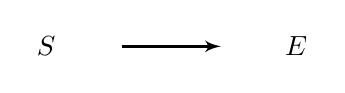
\begin{tikzpicture}[>=latex',line join=bevel,]
\pgfsetlinewidth{1bp}
\pgfsetcolor{black}

% Edge: S -> E
\draw [->] (54.403bp,18bp) .. controls (62.393bp,18bp) and (71.311bp,18bp)  .. (89.919bp,18bp);

% Node: S
\begin{scope}
  \definecolor{strokecol}{rgb}{0.0,0.0,0.0};
  \pgfsetstrokecolor{strokecol}
  \draw (27bp,18bp) node {$S$};
\end{scope}

% Node: E
\begin{scope}
  \definecolor{strokecol}{rgb}{0.0,0.0,0.0};
  \pgfsetstrokecolor{strokecol}
  \draw (117bp,18bp) node {$E$};
\end{scope}

\end{tikzpicture}

\caption[]{A  control flow graph for the empty \D{} program.}

\label{figure:cfg-empty}

\end{figure}



\subsection{Function clauses}

While node construction and destruction are primitive operations in \D{}, we'll
refrain ourselves from delving into such details in the control flow graphs of
our programs. Indeed because \emph{node construction and destruction always
terminates}. Instead, we'll let a \emph{function clause} define a point in a
program.

The expression of the clause can thereafter make calls to its
enclosing\footnote{We say that a function \emph{consists} of function clauses
and a function clause is \emph{enclosed} in a function.}, or some other
function. Such calls are represented by transfer of control, that is, arcs.
Disregarding the cases where a function clause expression makes multiple calls
to the same function with different arguments, these arcs need not be
disjunctively labelled since all of these transitions happen unconditionally as
a result of evaluating the expression. More specifically, \emph{we consider the
order of evaluation to be insignificant}, and hence undeserving of labelling.
We further discuss the reasons for this below.

If calls are separated by node construction, the order in which those calls are
made is definitely insignificant. For instance, consider the expression
\mono{(f a).(g b)}, where \mono{f} and \mono{g} are some well-defined
functions, $\text{\mono{f}}\neq\text{\mono{g}}$, and \mono{a} and \mono{b} are
some bound variables. It makes no difference to the final result which of the
calls, \mono{f a} and \mono{g b}, is evaluated first. Indeed, they can be
evaluated in parallel, and we would still get the same result. This is easy to
see for any nested construction of results of function calls, as in e.g.
\mono{(f a).0.(g b)}.

On the other hand, the syntax and semantics of \D{} allow for function calls to
be nested as in e.g. the expression \mono{(f (g a) (h b))}, where \mono{h} is
also some well-defined function and is pairwise unequal to \mono{f} and
\mono{g}. While the order of evaluation of \mono{g a} and \mono{h b} is
\emph{insignificant} wrt. to one another, as with function calls separated by
construction, the order of evaluation of these two subexpressions wrt. to the
call to function \mono{f}, \emph{is significant to the result}, and
\emph{might} be significant to termination analysis in general. However, we'll
regard this as insignificant for the time being for mere simplicity. We'll come
back to the question of whether size-change termination analysis can benefit
from regarding this as significant later on.

We can now draw a control flow graph for the program define in
\referToListing{cfg-sample-1} as shown in \referToFigure{cfg-sample-1}.

\begin{lstlisting}[label=listing:cfg-sample-1,caption={A sample \D{} program, always returning \mono{0.0.0}.}]
f x y := x.y
g _ := 0
h _ := 0
i x y := (f ((h y).(g x)) (h y))
i input input
\end{lstlisting}

\begin{figure}[htbp!]
\centering
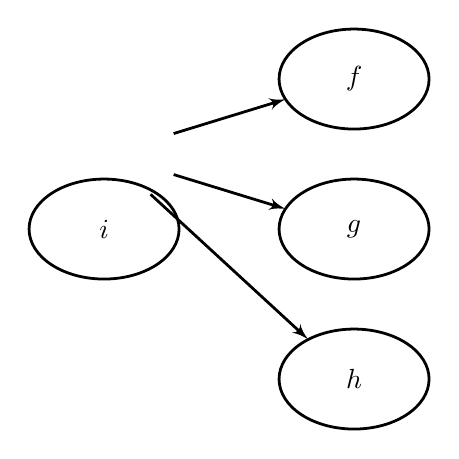
\begin{tikzpicture}[>=latex',line join=bevel,]
\pgfsetlinewidth{1bp}
\pgfsetcolor{black}

% Edge: i -> h
\draw [->] (133.73bp,84.519bp) .. controls (147.37bp,71.964bp) and (167.3bp,53.624bp)  .. (190.4bp,32.356bp);

% Edge: i -> f
\draw [->] (142.05bp,106.38bp) .. controls (151.44bp,109.26bp) and (162.36bp,112.61bp)  .. (182.29bp,118.72bp);

% Edge: i -> g
\draw [->] (142.05bp,91.622bp) .. controls (151.44bp,88.741bp) and (162.36bp,85.389bp)  .. (182.29bp,79.275bp);

% Node: g
\begin{scope}
  \definecolor{strokecol}{rgb}{0.0,0.0,0.0};
  \pgfsetstrokecolor{strokecol}
  \draw (207bp,72bp) ellipse (27bp and 18bp);
  \draw (207bp,72bp) node {$g$};
\end{scope}

% Node: f
\begin{scope}
  \definecolor{strokecol}{rgb}{0.0,0.0,0.0};
  \pgfsetstrokecolor{strokecol}
  \draw (207bp,126bp) ellipse (27bp and 18bp);
  \draw (207bp,126bp) node {$f$};
\end{scope}

% Node: i
\begin{scope}
  \definecolor{strokecol}{rgb}{0.0,0.0,0.0};
  \pgfsetstrokecolor{strokecol}
  \draw (117bp,72bp) ellipse (27bp and 18bp);
  \draw (117bp,72bp) node {$i$};
\end{scope}

% Node: h
\begin{scope}
  \definecolor{strokecol}{rgb}{0.0,0.0,0.0};
  \pgfsetstrokecolor{strokecol}
  \draw (207bp,18bp) ellipse (27bp and 18bp);
  \draw (207bp,18bp) node {$h$};
\end{scope}

\end{tikzpicture}

\caption[]{A  control flow graph for the \D{} program in
\referToListing{cfg-sample-1}. The graph does not explicitly specify
back-propagation of control, if any.}

\label{figure:cfg-sample-1}

\end{figure}



\subsection{Call cycles}

A call cycle occurs when there is a cyclical transition of control between the
nodes of a control flow graph. I.e. when there is a cycle in the control flow
graph.

\begin{lemma} We're concerned with call cycles in control flow graphs since
non-termination cannot occur if not for an infinite control flow cycle.
\end{lemma}

\begin{proof} If a program has a control flow graph with no cycles and does not
terminate, then one of the primitive operations, i.e. construction,
destruction, comparison or binding, does not terminate, which is certainly
absurd given the semantics of \D{}. \end{proof}

Call cycles in \D{} can occur in recursive or mutually recursive function
clauses.

We will henceforth refer to function clauses with recursive calls as
\emph{recursive clauses} and their counterparts, i.e. the base clauses of a
function declaration, \emph{terminal clauses}.

\subsection{Disregarding back-propagation}

It is worth noting that in \referToFigure{cfg-sample-1}, the clauses that make
no function calls have out-degree $0$. Technically, these functions \emph{do
transfer control} -- back to the callee. We may refer to this process as
\emph{back-propagation of control}. While considering back-propagation is
seemingly important to a concept that bases itself on the changes in the sizes
of the program values, we're only concerned with call cycles.

The thing with back-propagation is that forward-propagation after
back-propagation of a call cannot occur due to the way \D{} is defined. Hence,
what we are really concerned with is, ``how deep the rabbit hole goes'', before
we back-propagate, as back-propagation superimplies termination of the function
we're back-propagating out of.

\subsection{Dropping the start and end nodes}

The disregard of the back-propagation of control forces us to either redefine
the transition from the start node and the transitions to the end node. This is
because neither of these transitions are ever back-propagated, while all other
transitions \emph{must be} back-propagated if the program terminates.

Alternatively, disregard of back-propagation allows us to drop these nodes
completely and concentrate on the clauses and explicit calls within the clause
expressions. Hence, start and end nodes will not appear in any further graphs.

\subsection{Control flow graphs vs. abstract static call graphs}

Disregard of back-propagation allows us to consider control flow graphs
presented in this text as mere \emph{abstract static call graphs}, henceforth
referred to simply as, \emph{call graphs}. The abstraction applied to these
graphs compared to regular static call graphs is that the concrete arguments of
the function calls are not considered, and we merely consider how these values
can change in size from for a given function call. Interestingly, the problem
of termination analysis can be rephrased as the problem of determining whether
the regular static call graph of a program, i.e. the one containing the
concrete function arguments, is finite.

\subsection{Multiple calls to the same function}

Up until now we've only regarded expressions that don't make calls to the same
function with varying arguments. This is because these calls have to be
disjunctively labelled for the purposes of our analysis, because the use of
varying arguments \emph{may} mean varying decrease (or increase), in values for
the different calls within the expression. For this purpose we'll disjunctively
label \emph{all} the calls within an expression, if necessary, but remember
that this has nothing to do with evaluation order as has been discussed above.

This allows us to draw a control flow graph, or equivalently, a call graph,
for the program in \referToListing{cfg-sample-2}. Here, we've already
disjunctively labelled all of the calls in the expressions. This call graph is
drawn in \referToFigure{cfg-sample-2}.

\begin{lstlisting}[label=listing:cfg-sample-2,caption={A sample \D{} program, always returning \mono{(0.x).(0.y)}, where \mono{x} and \mono{y} are arbitrary \D{} values supplied by the user.}]
f x y := x.y
g x := 0.x
i x y := (0: f (1: g x) (2: g y))
i input input
\end{lstlisting}

\begin{figure}[htbp!]
\centering
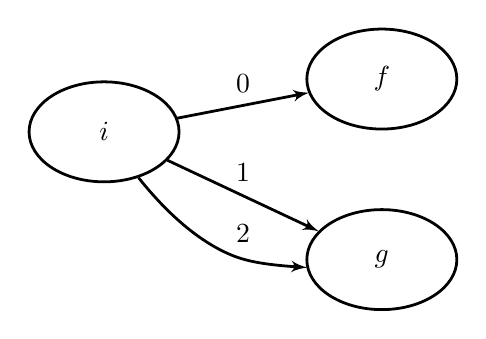
\begin{tikzpicture}[>=latex',line join=bevel,]
\pgfsetlinewidth{1bp}
\pgfsetcolor{black}

% Edge: i -> g
\draw [->] (141.75bp,53.791bp) .. controls (155.07bp,47.538bp) and (172.33bp,39.435bp)  .. (196.31bp,28.18bp);

\definecolor{strokecol}{rgb}{0.0,0.0,0.0};
\pgfsetstrokecolor{strokecol}
\draw (169bp,49.5bp) node {$1$};

% Edge: i -> g
\draw [->] (131.41bp,47.488bp) .. controls (139.3bp,37.571bp) and (150.73bp,25.786bp)  .. (164bp,20bp) .. controls (169.56bp,17.574bp) and (175.77bp,16.246bp)  .. (192.14bp,15.146bp);
\draw (169bp,27.5bp) node {$2$};

% Edge: i -> f
\draw [->] (145.24bp,68.893bp) .. controls (156.67bp,71.109bp) and (170.38bp,73.767bp)  .. (192.85bp,78.124bp);
\draw (169bp,81.5bp) node {$0$};

% Node: i
\begin{scope}
  \definecolor{strokecol}{rgb}{0.0,0.0,0.0};
  \pgfsetstrokecolor{strokecol}
  \draw (119bp,64bp) ellipse (27bp and 18bp);
  \draw (119bp,64bp) node {$i$};
\end{scope}

% Node: g
\begin{scope}
  \definecolor{strokecol}{rgb}{0.0,0.0,0.0};
  \pgfsetstrokecolor{strokecol}
  \draw (219bp,18bp) ellipse (27bp and 18bp);
  \draw (219bp,18bp) node {$g$};
\end{scope}

% Node: f
\begin{scope}
  \definecolor{strokecol}{rgb}{0.0,0.0,0.0};
  \pgfsetstrokecolor{strokecol}
  \draw (219bp,83bp) ellipse (27bp and 18bp);
  \draw (219bp,83bp) node {$f$};
\end{scope}
%
\end{tikzpicture}

\caption[]{A  control flow graph for the \D{} program in \referToListing{cfg-sample-2}.}

\label{figure:cfg-sample-2}

\end{figure}



\subsection{Multiple clauses}

If function clauses are nodes, and the function calls within the expressions of
the function clauses are unconditional transitions, what exactly happens if the
arguments supplied to the function clause fail to match the pattern declaration
for the clause?

The semantics of \D{} tell us to make an unconditional transition to the
immediately next clause of the function. There is at most one such transition
for any clause, and the last clause of a function declaration cannot fail to
pattern match\footnote{See \referToSection{d-sos}.}.

We'll refer to these transitions as \emph{fail transitions} and visually mark
them with a dotted line rather than a filled line. We need this way of visually
distinguishing fail transitions from the rest since they are conditionally
different, in that for any clause with a fail transition, either the fail
transition is chosen, or all the non-fail transitions are chosen
simultaneously.

Before we can draw the call graph we also need a way to distinguish the clauses
of a function wrt. the program text. We decide to enumerate the clauses
top-to-bottom starting with 0. Sometimes we'll annotate the program text with
these unique labels for each clause to make the call graph more readable.

Hence, we can now draw the call graph for the program defined in
\referToListing{cfg-loop} as shown in \referToFigure{cfg-loop}.

\begin{lstlisting}[label=listing:cfg-loop,caption={A simple, down-counting loop in \D{}.}]
f0: f 0 := 0
f1: f x._ := f x

f input
\end{lstlisting}

\begin{figure}[htbp!]
\centering
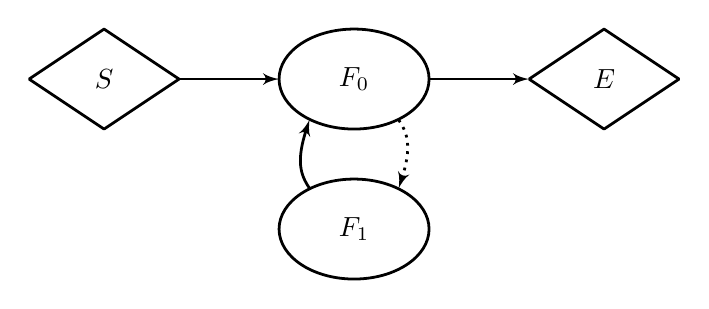
\begin{tikzpicture}[>=latex',line join=bevel,]

\pgfsetlinewidth{1bp}
\pgfsetcolor{black}

% Edge: F0 -> F1
\draw [->,dotted] (133.06bp,73.287bp) .. controls (136.46bp,68.306bp) and (137.79bp,63.325bp)  .. (133.09bp,48.766bp);

% Edge: S -> F0
\draw [->] (54.403bp,88bp) .. controls (62.393bp,88bp) and (71.311bp,88bp)  .. (89.919bp,88bp);

% Edge: F1 -> F0
\draw [->] (100.91bp,48.766bp) .. controls (97.522bp,53.747bp) and (96.204bp,58.727bp)  .. (100.94bp,73.287bp);

% Edge: F0 -> E
\draw [->] (144.4bp,88bp) .. controls (152.39bp,88bp) and (161.31bp,88bp)  .. (179.92bp,88bp);

% Node: F0
\begin{scope}
  \definecolor{strokecol}{rgb}{0.0,0.0,0.0};
  \pgfsetstrokecolor{strokecol}
  \draw (117bp,88bp) ellipse (27bp and 18bp);
  \draw (117bp,88bp) node {$F_0$};
\end{scope}

% Node: F1
\begin{scope}
  \definecolor{strokecol}{rgb}{0.0,0.0,0.0};
  \pgfsetstrokecolor{strokecol}
  \draw (117bp,34bp) ellipse (27bp and 18bp);
  \draw (117bp,34bp) node {$F_1$};
\end{scope}

% Node: S
\begin{scope}
  \definecolor{strokecol}{rgb}{0.0,0.0,0.0};
  \pgfsetstrokecolor{strokecol}
  \draw (27bp,106bp) -- (0bp,88bp) -- (27bp,70bp) -- (54bp,88bp) -- cycle;
  \draw (27bp,88bp) node {$S$};
\end{scope}

% Node: E
\begin{scope}
  \definecolor{strokecol}{rgb}{0.0,0.0,0.0};
  \pgfsetstrokecolor{strokecol}
  \draw (207bp,106bp) -- (180bp,88bp) -- (207bp,70bp) -- (234bp,88bp) -- cycle;
  \draw (207bp,88bp) node {$E$};
\end{scope}

\end{tikzpicture}

\caption[]{A  control flow graph for the program defined in
\referToListing{d-loop}.}

\label{figure:cfg-loop}

\end{figure}

 

For a more complex example, let's consider the call graph for the program
\mono{reverse} introduced in \referToSection{d-samples}. The program is
repeated in annotated form in \referToListing{cfg-reverse}, and its
corresponding call graph is shown in \referToFigure{cfg-reverse}.

\begin{lstlisting}[label=listing:cfg-reverse,caption={An annotated version of the program \mono{reverse} introduced in \referToSection{d-samples}.}]
r0: reverse 0 := 0
r1: reverse left.right := (0: reverse right).(1: reverse left)

reverse input
\end{lstlisting}

\begin{figure}[htbp!]
\centering
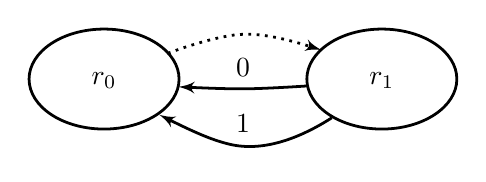
\begin{tikzpicture}[>=latex',line join=bevel,]
\pgfsetlinewidth{1bp}
\pgfsetcolor{black}

% Edge: R0 -> R1
\draw [->,dotted] (49.969bp,34.268bp) .. controls (56.882bp,36.851bp) and (64.635bp,39.282bp)  .. (72bp,40.58bp) .. controls (79.767bp,41.948bp) and (88bp,40.866bp)  .. (105.24bp,35.467bp);

% Edge: R1 -> R0
\draw [->] (99.957bp,22.51bp) .. controls (94.056bp,22.123bp) and (87.816bp,21.778bp)  .. (82bp,21.58bp) .. controls (76.252bp,21.384bp) and (70.164bp,21.454bp)  .. (53.809bp,22.204bp);

\definecolor{strokecol}{rgb}{0.0,0.0,0.0};
\pgfsetstrokecolor{strokecol}
\draw (77bp,29.08bp) node {$0$};

% Edge: R1 -> R0
\draw [->] (108.98bp,11.053bp) .. controls (98.589bp,4.4007bp) and (84.865bp,-1.5798bp)  .. (72bp,1.5798bp) .. controls (66.559bp,2.9161bp) and (61.044bp,5.0566bp)  .. (46.908bp,12.145bp);
\draw (77bp,9.0798bp) node {$1$};

% Node: R0
\begin{scope}
  \definecolor{strokecol}{rgb}{0.0,0.0,0.0};
  \pgfsetstrokecolor{strokecol}
  \draw (27bp,25bp) ellipse (27bp and 18bp);
  \draw (27bp,24.58bp) node {$r_0$};
\end{scope}

% Node: R1
\begin{scope}
  \definecolor{strokecol}{rgb}{0.0,0.0,0.0};
  \pgfsetstrokecolor{strokecol}
  \draw (127bp,25bp) ellipse (27bp and 18bp);
  \draw (127bp,24.58bp) node {$r_1$};
\end{scope}
%
\end{tikzpicture}

\caption[]{A  control flow graph for the \D{} program in \referToListing{cfg-reverse}.}

\label{figure:cfg-reverse}

\end{figure}
 

\subsection{Deeply nested function calls}

Blah

\section{Size-change termination principle}

Consider the program in \referToListing{cfg-loop} and it's corresponding call
graph in \referToFigure{cfg-loop}. Without any further information about the
control transitions, the program seemingly loops indefinitely. However, there
are some things that we can deduce about the control transitions.

\begin{lemma} If we can deduce for every control flow cycle in a prorgram that
it reduces a value of well-founded data-type on each iteration of the cycle,
then the value must eventually bottom out and the program must terminate.
\end{lemma}

\begin{proof} Assume for the sake of contradiction that a program that reduces
a value of a well-founded data type in each call cycle does not terminate.
Then, either the value reduces indefinitely, which is a contradiction to the
well-foundedness of its data type, or some noncyclic call sequence causes an
infinite loop, also an absurdity due to the definition of \D{}. \end{proof}

That is the \emph{size-change termination principle}. All values in \D{} are
inherently well-founded so what remains to be shown is how we can deduce from a
call cycle whether it reduces a value on each iteration.

\begin{lemma}\label{lemma:cycle-reduce} A control flow cycle reduces a value on
each iteration if at least one of the participating control transitions reduces
the value and all other control transitions do not increase that
value.\end{lemma}

\begin{proof} If a value is not reduced in a cycle, it either stays the same or
is increased. If it is increased, then at least one control transition must've
increased the value, an absurdity. If it stays the same then none of the
participating control transitions have neither increased nor decreased the
value, also an absurdity. \end{proof}

By the definition of call graphs, function clauses participate as nodes in a
call cycle. A control transition is a directed edge between two function
clauses where one clause is the \emph{source} and the other is the
\emph{target}. 

We can analyze how a value changes it's size through a call sequence by
analyzing the size relation between the variables bound in the source and the
variables bound in the target of every control transition.

\begin{definition} The relation $\Phi\ :\ C_{caller} \times C_{callee} \times
N_{caller} \times N_{callee} \rightarrow \{\bot,<,\leq\}$ is defined to be the
size relation between the caller and callee
clauses in \D{} where $N_{caller}$ are the names of the variables bound in the
caller, and $N_{callee}$ are the names of the variables bound in the callee.
Note, that we are only concerned with reductions and non-increases in size, all
other relationships are marked by the no relationship symbol $\bot$. Initially,
the relationship between all the clauses and their variables is $\bot$.
\end{definition}

The construction of the relationship $\Phi$ for a given transition depends
first and foremost on whether that transition is a fail or success transition.

\subsection{Fail transitions}

A fail transition occurs if the values passed to a given clause to match it's
pattern. If the values fail to match the pattern, no variables are bound and
hence no change in values can occur. The values are simply passed along as they
were to the next clause of the function declaration.

\begin{lemma} Fail transitions are transitive in the sense that the
relationship between the variables bound in the source and the variables bound
in the target is the same regardless of the number of fail transitions in
the path between the source and the target.\end{lemma}

\begin{proof} Follows from the semantics of \D{}. \end{proof}

We are not concerned with exact equivalence, hence all fail transitions in the
$\Phi$ relation return the relation $\leq$ for all variable pairs.

Note, that due to \D{} being first order and statically scoped, the variable
space is always initially empty when a function clause begins pattern matching.

\subsection{Success transitions}

Since \D{} is a call-by-value language, when a function call is encountered,
the source evaluates the arguments of the function call and generates some
\emph{values} before giving up control.

The values may hence be a nested construction of some concrete values, values
bound to variables in the source, and results of nested function calls. Without
further regard of nested function calls, this implies that a \emph{size
relation} can be deduced between the variables bound in the source and the
values that result from an evaluation of the function call arguments. 

Of course, we cannot deduce a precise size displacement as the values of the
bound variables may initially be \emph{unknown} at compile
time\footnote{Although some values can be deduced via static analysis of the
program, others can come in from the outside world via the 0-ary function
\mono{input} at run time.}.  However, we can deduce a \emph{safe} displacement
estimate, such that it is less than or equal to the actual displacement in
terms of absolute value. For instance, if the expression \mono{a.b} appears as
a function call argument, where \mono{a} and \mono{b} are some bound variables
with unknown values, and this argument evaluates to some value $v$, then we can
\emph{safely} say that $v>\text{\mono{a}}$, $v>\text{\mono{b}}$,
$v\geq\text{\mono{a.0}}$ and $v\geq\text{\mono{0.b}}$.

We decide to ignore the nested function calls because this would imply a more
complex static analysis of the program. Specifically, we're unable to say
anything about the result of the nested function call from the scope of the
source clause alone. Instead, we treat results from nested function calls
simply as variables with \emph{unknown} values. We also make sure to keep these
variables separate from the bound variables as there is no relationship to draw
between these ``variables'' and the variables bound in the
target\footnote{While this information may be useful for dead-code elimination
and other forms of static analysis, this is of little importance to size-change
termination.}.

More formally, given a function argument as the expression $x$, we construct
the expression $x^s$ where we replace all first-level nested function
calls\footnote{Nested function calls of nested function calls are hence
considered irrelevant to the derivation of the size relation of the top-level
call, however, they may become relevant as we derive the size relations of the
corresponding nested calls.} by auxiliary variables.  We group all those
auxiliary variables into the set of variable names $N_{calls}^s$ and all the
remaining variables into the set $N_{vars}^s$.  Furthermore we construct the
auxiliary variable names in such way that $N_{vars}^s\cup
N_{calls}^s=\emptyset$.  Hence, we obtain the tuple
$(x^c,N_{vars}^s,N_{calls}^s)$.

Continuing on with the example above, i.e. having the size relations
$\{v>\textt{a}, v> \textt{b}, v\geq \textt{a.0}, v\geq \textt{0.b}\}$, assume
that the target clause has the corresponding pattern \mono{x.y}. The question
henceforth is how do we draw the relationship that $\textt{a}\equiv\textt{x}$
and $\textt{b}\equiv\textt{y}$, or perhaps simply that the control transition
neither decreases nor increases any values. We can perform a corresponding
analysis on the pattern declaration and deduce the set of conditions that will
hold after pattern matching succeeds, indeed, $\{v>\textt{x}, v> \textt{y},
v\geq \textt{x.0}, v\geq \textt{0.y}\}$. The participation of $x$ in the same
kind of relations as $a$, and the participation of $y$ in the same kind of
relations as $b$, does not alone indicate their respective equivalence, since
the actual property that $v\equiv\textt{a.b}$ is lost.

On the other hand, if we had to formally define the relation that had to be
built between the variables bound in the source and the values that the
function call arguments evaluated to, this would be a relation between values
and some kind of ``abstract patterns'', as e.g. $v\geq\textt{0.b}$.

To simplify the entire process, instead of deducing actual size relations
between the variables bound in the source and the values that the function
arguments evaluate to, we can simply turn the function argument into the
abstract pattern to begin with. The actual size relations are hence withkept
and can be deduced at a later stage in the process.

Indeed, the tuple $(x^s,N_{vars}^s,N_{calls}^s)$ constitutes such an abstract
pattern already, since the expression $x^s$, contains no function calls and
hence syntactically matches a pattern in \D{}\footnote{See
\referToSection{d-syntax} if you're uncertain.}. We henceforth refer to such an
expression as $p^s$\footnote{Where $s$ stands for \emph{source}.}. Given a
clause with the pattern $p^t$\footnote{Where $t$ stands for \emph{target}.}, we
can easily deduce the set $N_{vars}^t$, which is the set of variable names used
in $p$. Our task is then to deduce a size relation between the variables in the
sets $N_{vars}^s$ and $N_{vars}^t$ given the tuples
$(p^s,N_{vars}^s,N_{calls}^s)$ and $(p^t,N_{vars}^t)$.

\subsection{Pattern matching}

Let the function $\phi\ :\ \mathbb{N} \times \mathbb{N} \rightarrow
\{<,\leq,\bot\}$ denote the function $\lambda N^t, N^s .
\Phi\left(C^t,C^s,N^t,N^s\right)$. In the following section we will discuss the
rules involved in deducing the function $\phi$, that is, the function $\Phi$
for some given source and target of a success transition.

For this purpose we will regard the tuples $(P^s,N_{vars}^s)$ and
$(P^t,N_{vars}^t)$, of a given success transition, where $P^s$ is the list of
abstract patterns derived from the function arguments in the source, and $P^t$
is the list of corresponding actual patterns in the target. Furthermore, let
$N_{vars}^s$ and $N_{vars}^t$ be unary functions of the type
$\mathbb{P}\rightarrow\mathbb{N}^*$, accepting a pattern and yielding the
variable names that are contained both in the input pattern and the sets
$N_{vars}^s$ and $N_{vars}^t$, respectively.

In the following analysis we will look at but one instance of the lists $P^s$
and $P^t$, namely the abstract pattern $p^s$ from the source and its
corresponding actual pattern in the declaration, $p^t$. In total, however, this
process has to be repeated for each such pair given the sets $P^s$ and $P^t$,
iteratively extending the definition of the relation $\phi$ to all variables
bound in the sets $N_{vars}^s$ and $N_{vars}^t$.

We initially define $\phi$ to yield the value $\bot$ for all arguments. We will
continuously modify this definition as we process $p^s$ and $p^t$. We denote
this within the semantics in a manner similar to the state $\sigma$ in the
semantics\footnote{See \referToSection{d-sos}.}. However, $\phi$ is now a
binary ``memory'', requiring both a target name and a source name (in that
order). For simplicity, we will borrow some suger coding from the matlab
notation which allows us to provide a collection in place of a single element
and let the runtime apply the given function to each element in the collection.
For instance, we might write that $\phi\left(N_{vars}^t(p^t), n^s\right)\mapsto
<$, meaning that all the target variables used in $p^t$ are strictly less than
the source variable $n^s$.

We now define a summoning rule, dividing the rules up into sub-rules:

\begin{equation}
{
    \left\langle\proc{A},p^t,p^s,\phi\right\rangle
    \rightarrow
    \phi'
  \vee
    \left\langle\proc{B},p^t,p^s,\phi\right\rangle
    \rightarrow
    \phi'
  \vee
    \left\langle\proc{C},p^t,p^s,\phi\right\rangle
    \rightarrow
    \phi'
  \vee
    \left\langle\proc{D},p^t,p^s,\phi\right\rangle
    \rightarrow
    \phi'
  \vee
    \left\langle\proc{E},p^t,p^s,\phi\right\rangle
    \rightarrow
    \phi'
}\over{
  \left\langle p^t,p^s,\phi\right\rangle
  \rightarrow
  \phi'
}
\end{equation}

One of the simpler cases is when the abstract pattern $p^s$ is simply \mono{0},
or some name $n^s$, and $n^s\in N_{calls}^s$. Since no variables bound in the
source participate in $p^s$, then no relations need to be drawn to any of the
target variables that might appear in the corresponding $p^t$. Hence, $\phi$
need not be modified.

\begin{equation}\label{eq:sct-pattern-source-fail}
{
\left(
    p^s\rightarrow 0
  \vee
\left(
    p^s\rightarrow n^s
  \wedge
    n^s\notin N_{vars}^s
\right)
\right)
  \wedge
    \phi\rightarrow\phi'
}\over{
  \left\langle\proc{A},p^t,p^s,\phi\right\rangle
  \rightarrow
  \phi'
}
\end{equation}

This has a symmetrical case. Indeed when $p^t$ is neither a destruction, nor
any name $n^t$, that is, it is \mono{\_} or \mono{0}. This pattern contains no
variables, and hence  no relations need to be drawn from any of the variables
that might appear in the corresponding $p^s$. Hence, $\phi$ need not be
modified in such a case either.

\begin{equation}
{
\left(
    p^t\rightarrow 0
\vee
    p^t\rightarrow \_
\right)
  \wedge
    \phi\rightarrow\phi'
}\over{
  \left\langle\proc{B},p^t,p^s,\phi\right\rangle
  \rightarrow
  \phi'
}
\end{equation}

If $p^t$ is the name pattern $n^t$, the matters get a bit more complicated:

\begin{enumerate}

\item If $p^s$ is some node, then all the variables that occur in $p^s$, i.e.
$N_{vars}^s(p^s)$, will all be strictly less than $n^t$ by the semantics of
\D{}. However, we are not concerned with this relation, as we would like to
know when a value is decreased from source to target, and not, as in this case,
increased.

\item If $p^s$ is also some name pattern $n^s$, and  $n^s\in N^s_{vars}$, then
the values of these corresponding variables will be \emph{equivalent}. However,
we're not concerned with exact equivalence, and simply mark this relationship
with the weaker, but still sound relation, $\leq$:

\begin{equation}
{
    p^t\rightarrow n^t
  \wedge
    p^s\rightarrow n^s
  \wedge
    n^s\in N_{vars}^s
  \wedge
    \left\langle\phi\left(n^t, n^s\right)\mapsto \leq\right\rangle\rightarrow\phi'
}\over{
  \left\langle\proc{C},p^t,p^s,\phi\right\rangle
  \rightarrow
  \phi'
}
\end{equation}

\end{enumerate}

If $p^t$ is a destruction and $p^s$ is the variable name $n^s$, then we can safely say that
all the variables that occur in $p^t$, i.e. $N_{vars}^t(p^t)$, are all strictly less
than the variable in $n^s$:

\begin{equation}
{
    p^t\rightarrow p^t_1\cdot p^t_2
  \wedge
    p^s\rightarrow n^s
  \wedge
    n^s\in N_{vars}^s
  \wedge
    \left\langle\phi\left(N_{vars}^t(p^t), n^s\right)\mapsto <\right\rangle\rightarrow\phi'
}\over{
  \left\langle\proc{D},p^t,p^s,\phi\right\rangle
  \rightarrow
  \phi'
}
\end{equation}

If both $p^t$ and $p^s$ are a destructions, then the following recursive rule applies:

\begin{equation}
{
    p^t\rightarrow p^t_1\cdot p^t_2
  \wedge
    p^s\rightarrow p^s_1\cdot p^s_2
  \wedge
    \left\langle p^t_1, p^s_1, \phi\right\rangle
    \rightarrow
    \phi''
  \wedge
    \left\langle p^t_2, p^s_2, \phi''\right\rangle
    \rightarrow
    \phi'
}\over{
  \left\langle\proc{E},p^t,p^s,\phi\right\rangle
  \rightarrow
  \phi'
}
\end{equation}

\section{Graph annotation}

Hence, we can deduce from \referToListing{cfg-loop}, that when $f_1$ makes a
call to $f_0$ it does so with a value strictly less then it's own argument,
i.e. the transition $f_1\rightarrow f_0$ strictly decreases a value. Visually
we will mark this with a $\downarrow$. The Lemmas \refer{lemma:d-pattern-leq}
and \refer{lemma:d-pattern-less} can be used to deduce the same sort of
relationship for the transitions $r_1\xrightarrow{0,1} r_0$ for
\referToListing{cfg-reverse}. These observations are summarised in
\referToFigure{sct-first}.

\begin{figure}[htbp!]
\centering

\subfigure[The program in \referToListing{cfg-loop}.]{
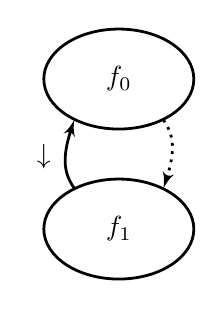
\begin{tikzpicture}[>=latex',line join=bevel,]

\pgfsetlinewidth{1bp}
\pgfsetcolor{black}

% Edge: F0 -> F1
\draw [->,dotted] (133.06bp,73.287bp) .. controls (136.46bp,68.306bp) and (137.79bp,63.325bp)  .. (133.09bp,48.766bp);

\draw (90bp,60bp) node {$\downarrow$};

% Edge: F1 -> F0
\draw [->] (100.91bp,48.766bp) .. controls (97.522bp,53.747bp) and (96.204bp,58.727bp)  .. (100.94bp,73.287bp);

% Node: F0
\begin{scope}
  \definecolor{strokecol}{rgb}{0.0,0.0,0.0};
  \pgfsetstrokecolor{strokecol}
  \draw (117bp,88bp) ellipse (27bp and 18bp);
  \draw (117bp,88bp) node {$f_0$};
\end{scope}

% Node: F1
\begin{scope}
  \definecolor{strokecol}{rgb}{0.0,0.0,0.0};
  \pgfsetstrokecolor{strokecol}
  \draw (117bp,34bp) ellipse (27bp and 18bp);
  \draw (117bp,34bp) node {$f_1$};
\end{scope}

\end{tikzpicture}
}

\subfigure[The program in \referToListing{cfg-reverse}.]{
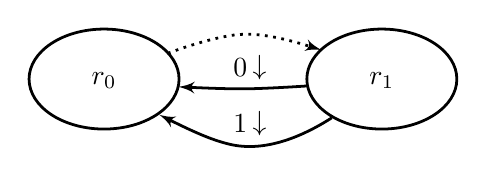
\begin{tikzpicture}[>=latex',line join=bevel,]
\pgfsetlinewidth{1bp}
\pgfsetcolor{black}

% Edge: R0 -> R1
\draw [->,dotted] (49.969bp,34.268bp) .. controls (56.882bp,36.851bp) and (64.635bp,39.282bp)  .. (72bp,40.58bp) .. controls (79.767bp,41.948bp) and (88bp,40.866bp)  .. (105.24bp,35.467bp);

% Edge: R1 -> R0
\draw [->] (99.957bp,22.51bp) .. controls (94.056bp,22.123bp) and (87.816bp,21.778bp)  .. (82bp,21.58bp) .. controls (76.252bp,21.384bp) and (70.164bp,21.454bp)  .. (53.809bp,22.204bp);

\definecolor{strokecol}{rgb}{0.0,0.0,0.0};
\pgfsetstrokecolor{strokecol}

\draw (76bp,29.08bp) node {$0$};
\draw (83bp,29.08bp) node {$\downarrow$};

% Edge: R1 -> R0
\draw [->] (108.98bp,11.053bp) .. controls (98.589bp,4.4007bp) and (84.865bp,-1.5798bp)  .. (72bp,1.5798bp) .. controls (66.559bp,2.9161bp) and (61.044bp,5.0566bp)  .. (46.908bp,12.145bp);

\draw (76bp,9.0798bp) node {$1$};
\draw (83bp,9.0798bp) node {$\downarrow$};

% Node: R0
\begin{scope}
  \definecolor{strokecol}{rgb}{0.0,0.0,0.0};
  \pgfsetstrokecolor{strokecol}
  \draw (27bp,25bp) ellipse (27bp and 18bp);
  \draw (27bp,24.58bp) node {$r_0$};
\end{scope}

% Node: R1
\begin{scope}
  \definecolor{strokecol}{rgb}{0.0,0.0,0.0};
  \pgfsetstrokecolor{strokecol}
  \draw (127bp,25bp) ellipse (27bp and 18bp);
  \draw (127bp,24.58bp) node {$r_1$};
\end{scope}
%
\end{tikzpicture}
}

\caption[]{Call graphs with annotated edges for various programs.}

\label{figure:sct-first}

\end{figure}


\subsection{Calls to multivariate functions}

The call graph notation used thus far has only been used for describing calls
to unary functions. As an example of a multivariate function, we may consider
the function \mono{normalized-less/2}, introduced in
\referToSection{d-size-less}. We use this function to define the program in
\referToListing{sct-normalized-less}. The corresponding call graph is shown in
\referToFigure{sct-normalized-less}.

\begin{lstlisting}[
  label={listing:sct-normalized-less},
  caption={A sample program with a multivariate function.}]
n0: normalized-less 0 b := b
n1: normalized-less _ 0 := 0
n2: normalized-less _.a _.b := normalized-less a b
normalized-less input input
\end{lstlisting}

\begin{figure}[htbp!]
\centering
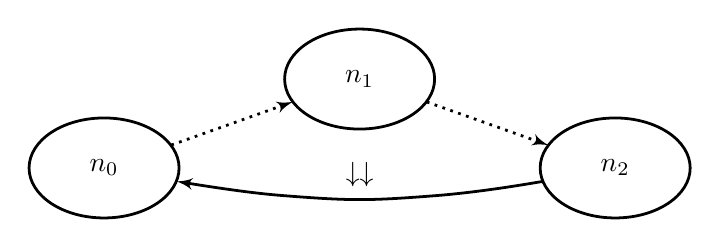
\begin{tikzpicture}[>=latex',line join=bevel,]
\pgfsetlinewidth{1bp}
\pgfsetcolor{black}

% Edge: n0 -> n1
\draw [->,dotted] (51.177bp,26.241bp) .. controls (61.57bp,29.936bp) and (74.012bp,34.36bp)  .. (94.901bp,41.787bp);

% Edge: n1 -> n2
\draw [->,dotted] (143.18bp,41.759bp) .. controls (153.57bp,38.064bp) and (166.01bp,33.64bp)  .. (186.9bp,26.213bp);

% Edge: n2 -> n0
\draw [->] (184.88bp,13.152bp) .. controls (173.12bp,11.121bp) and (158.89bp,9.0013bp)  .. (146bp,8bp) .. controls (122.07bp,6.1419bp) and (115.93bp,6.1419bp)  .. (92bp,8bp) .. controls (82.632bp,8.7275bp) and (72.561bp,10.045bp)  .. (53.124bp,13.152bp);

\definecolor{strokecol}{rgb}{0.0,0.0,0.0};
\pgfsetstrokecolor{strokecol}
\draw (119bp,15.5bp) node {$\downarrow\downarrow$};

% Node: n0
\begin{scope}
  \definecolor{strokecol}{rgb}{0.0,0.0,0.0};
  \pgfsetstrokecolor{strokecol}
  \draw (27bp,18bp) ellipse (27bp and 18bp);
  \draw (27bp,18bp) node {$n_0$};
\end{scope}

% Node: n1
\begin{scope}
  \definecolor{strokecol}{rgb}{0.0,0.0,0.0};
  \pgfsetstrokecolor{strokecol}
  \draw (119bp,50bp) ellipse (27bp and 18bp);
  \draw (119bp,50bp) node {$n_1$};
\end{scope}
% Node: n2
\begin{scope}
  \definecolor{strokecol}{rgb}{0.0,0.0,0.0};
  \pgfsetstrokecolor{strokecol}
  \draw (211bp,18bp) ellipse (27bp and 18bp);
  \draw (211bp,18bp) node {$n_2$};
\end{scope}
%
\end{tikzpicture}

\caption[]{A  control flow graph for the program defined in
\referToListing{sct-normalized-less}.}

\label{figure:sct-normalized-less}

\end{figure}



The notation is straightforward, the juxtaposition of the $\downarrow$
indicates the size change of the respective arguments, read left to right as in
the function clause definition.

\subsection{Nonincreasing transitions}

There are cases where for a given transition in a call cycle, we can't tell
whether the sizes are strictly decreased or remain the same, but we can
definitely say that there is \emph{no increase} in the sizes of variables. As
an example, consider the program in \referToListing{sct-non-reducing}.

\begin{lstlisting}[
  label=listing:sct-non-reducing,
  caption={The binary function \mono{g} has a call cycle with nonincreasing
    sizes in variables.}]
g0: g 0 0 = 0
g1: g _.a b._ = g 0.a b.0
g input input
\end{lstlisting}


For the recursive clause $g_1$, it is unclear whether the sizes of the
variables are decreased in the transition $g_1\rightarrow g_0$, or not.
Specifically, if the arguments to \mono{g} are of the form \mono{0.\_} and
\mono{\_.0}, respectively, the size is \emph{not} decreased by the call. We'll
denote such transitions by the symbol $\Downarrow$. We can now draw the call
graph for the program in \referToListing{sct-non-reducing} as in
\referToFigure{sct-non-reducing}.

\begin{figure}[htbp!]
\centering
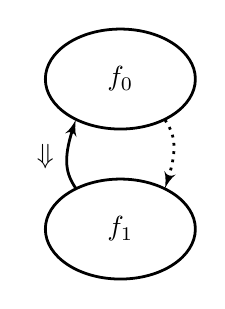
\begin{tikzpicture}[>=latex',line join=bevel,]

\pgfsetlinewidth{1bp}
\pgfsetcolor{black}

% Edge: F0 -> F1
\draw [->,dotted] (133.06bp,73.287bp) .. controls (136.46bp,68.306bp) and (137.79bp,63.325bp)  .. (133.09bp,48.766bp);

\draw (90bp,60bp) node {$\Downarrow$};

% Edge: F1 -> F0
\draw [->] (100.91bp,48.766bp) .. controls (97.522bp,53.747bp) and (96.204bp,58.727bp)  .. (100.94bp,73.287bp);

% Node: F0
\begin{scope}
  \definecolor{strokecol}{rgb}{0.0,0.0,0.0};
  \pgfsetstrokecolor{strokecol}
  \draw (117bp,88bp) ellipse (27bp and 18bp);
  \draw (117bp,88bp) node {$f_0$};
\end{scope}

% Node: F1
\begin{scope}
  \definecolor{strokecol}{rgb}{0.0,0.0,0.0};
  \pgfsetstrokecolor{strokecol}
  \draw (117bp,34bp) ellipse (27bp and 18bp);
  \draw (117bp,34bp) node {$f_1$};
\end{scope}

\end{tikzpicture}

\caption[]{An annotated call graph for the program in \referToListing{sct-non-reducing}.}

\label{figure:sct-non-reducing}

\end{figure}


\subsection{Increasing transitions}


%Values are not always decreasing.

%Consider the following program:

\begin{lstlisting}[
  label=listing:sct-infinite-join,
  caption={The function \mono{infinite-join/2} infinitely joins..}]
f0: f a b = f a.b b.a
f input input
\end{lstlisting}

%The function clause expression constructs a new value by joining the two
%incoming arguments into a new node. While we're unable to say by how much the
%values are increased exactly, we know that both values are increased by at
%least 1 due to the creation of a node for each argument.


%\newpage

%A derrivable property from the program text is that the value sent as the
%argument in the transition $F_1\rightarrow F_0$ is \emph{always} strictly less
%than the value sent as the argument in the preceeding transition,
%$F_0\rightarrow F_1$. Additionally, we can universally state that \emph{false
%transitions from case nodes by definition can't change any values}. Hence, the
%infinite control flow sequence $F_0\rightarrow F_1\rightarrow F_0$ strictly
%decreases a well founded value in every iteration of the control flow cycle.
%This means that eventually the value bottoms out at $0$ which would validate
%the $F_0$ pattern and lead the program to terminate. In general, we can state
%the following:

%\begin{lemma}

%An infinite control flow sequnece infinitely decreases a well founded value if
%all the transitions in the corresponding control flow graph cycle either
%strictly decrease a value or keep all values unchanged, and at least one
%transition strictcly decreases a value.

%\end{lemma}

%\referToFigure{cfg-loop-down} showcases an edge-labelled control flow graph for
%\referToListing{d-loop}. Transitions for which we can \emph{safely} say that a
%value is decreased we mark with the symbol $\downarrow$, transitions for which
%we can \emph{safely} say that no value is increased we mark with the symbol
%$\top$. The graph is rather verbose and in future graphs we'll omit $\top$
%labels for nodes that universally can't increase a value, i.e. $S\rightarrow
%F_0$, $F_0\rightarrow E$ and $F_0\rightarrow F_1$.

%We can further prove the soundness of the size-change termination principle.

%\begin{proof} Assume for the sake of contradiction that there exists an
%infinite control flow sequence that infinitely decreases a well-founded data
%value. Assume furthermore that the program does not terminate. Then, some
%variable has to decrease indefinately, which contradicts with the definition of
%well-founded values. \end{proof}

%Unfortunately, this particular program can be trivially unfolded into a loop
%program, so the point of using size-change termination analysis may seem
%superflous. Indeed, the only change wrt. the control flow diagram is the
%notaiton used in the diagram. For such programs, the termination property is
%easily derrivable\cite{complexity-of-loop-programs}. 


\chapter{Shape-Change Termination}

Size-change termination, despite being simple is powerful enough to determine
the halting property for a large class of programs. Many authors have extended
the principle to even wider classes of programs, e.g. extending it to handle
initially not well-founded data types \cite{bound-analysis}, 

One trouble with size-change termination as described in the previous chapter
is \referToLemma{cycle-reduce}. This lemma makes size-change termination weak
in the sense that the overall shape changes in a given call cycle are
\emph{not} considered, and instead, call cycles are constrained to
monotonically decreasing call cycles.  However, there may be programs that have
calls, or even call cycles, that in terms of size, increase a value for a
finite amount of time, until some condition is met, or as in the case of \D{},
a value has some particular shape.

Consider the program in \referToListing{size-change-fail} as an example of a
program for which regular size-change termination is unable to determine the
halting property, while the property itself would seem fairly simple to deduce.
This is a sample program where some value is increased in terms of size in a
call cycle, but only until the value matches a certain shape, the shape
required by a terminal clause.

\begin{lstlisting}[
  label=listing:size-change-fail,
  caption={A terminating program with a call cycle where a value is
  temporarily increased.}]
$f_0$: f a.b.c.d := a
$f_1$: f a := f a.0
f input
\end{lstlisting}

The extension proposed in this chapter is to be able to determine the halting
property for such a class of programs without reducing size of the class of
programs for which size-change termination can already deduce the halting
property.

In the discussion below we continue the assumptions from
\referToSection{size-change-termination}. In particular, all clauses in a
program are unary and bind at most one variable. Also, we can safely disregard
terminal clauses in call graphs.

\section{The class of programs considered}

Before we can speak of extending size-change termination to determine the
halting property for programs in the same class as
\referToListing{size-change-fail}, we need to formally define that class.

Actual conditions in \D{} can only be expressed in terms of patterns in
function clauses. Hence, we disregard programs that rely on equality or size
comparison conditions for termination, since this type of programs will often
already be covered by regular size-change termination, and if not, they at the
very least come down to recursive pattern matching.

As an example of a program where size-change termination is already prevalent,
consider a program that finds the $n^{th}$ Fibonacci number as the one already
presented in \referToSection{d-samples}. The function \mono{fibonacci-aux}
seemingly increases a value until a condition is met, in particular, until we
count one of the arguments down to \mono{0}. However, due to the fact that we
count that we decrease the value of that argument in \emph{recursive} clause of
the \mono{fibonacci-aux} functions, the halting property is certainly already
deducible by regular size-change termination.

Instead, we turn our attention to simpler programs, ones that rely solely on
conditions defined in terms of patterns. Consider again the program in
\referToListing{size-change-fail}. The function \mono{f} has only one terminal
clause, the one that accepts a shape as in \referToFigure{size-change-fail-f0}.
If the function argument has any other shape, i.e. either a shape as in
\referToFigure{size-change-fail-f1-0}, \referToFigure{size-change-fail-f1-1} or
\referToFigure{size-change-fail-f1-2}, then the recursive clause $f_1$ is
chosen. For any argument $b\in\mathbb{B}$, the clause $f_1$ replaces the
right-most child of the value, which is always \mono{0}, with a node.

For instance, the smallest possible argument $b\in\mathbb{B}$ is \mono{0}.  If
passed such a value, $f_1$ transforms it into a value that has a shape that
corresponds to \referToFigure{size-change-fail-f1-1}, which in turn transforms
the value into one that matches \referToFigure{size-change-fail-f1-2}, which in
turn transforms the value into one that matches
\referToFigure{size-change-fail-f0}, i.e. the terminal clause. What's more,
there are infinitely many other values that will match the shape
\referToFigure{size-change-fail-f1-1}, and for each of them, the clause $f_1$
will transform them into values that match
\referToFigure{size-change-fail-f1-2}, which will transform them into values
that match \referToFigure{size-change-fail-f0}.

\includeFigure{size-change-fail-f0}{The shape that the clause $f_0$ in
\referToListing{size-change-fail} will accept.}

\begin{figure}[htbp!]
\begin{minipage}{0.3\linewidth}
\centering

\includegraphics{figures/size-change-fail-f1-0}
\caption[]{The pattern \mono{0}.}
\label{figure:size-change-fail-f1-0}
\end{minipage}
\begin{minipage}{0.3\linewidth}
\centering
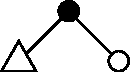
\includegraphics{figures/size-change-fail-f1-1}
\caption[]{The pattern \mono{a.0}.}
\label{figure:size-change-fail-f1-1}
\end{minipage}
\begin{minipage}{0.3\linewidth}
\centering
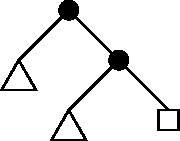
\includegraphics{figures/size-change-fail-f1-2}
\caption[]{The pattern \mono{a.b.0}.}
\label{figure:size-change-fail-f1-2}
\end{minipage}
\end{figure}

We shall henceforth say that a clause such as $f_1$ changes the shape of any
argument $b$ to \emph{eventually} match the shape corresponding to a pattern of
the terminal clause $f_0$. The task then becomes to determine for each call
cycle in a program whether it changes the shape of the argument to eventually
match some terminal clause.

\section{Preliminaries}

Before we continue with this extension we can make a few important observations
based on the semantics of function clauses in \D{}.

\subsection{Deducing leafs}\label{section:extend-deducing-zero}

The \mono{.} operator in the patterns of function clauses in \D{} is
right-associative. Hence, a pattern of the form \mono{a.b.c.d} is the same as
\mono{a.(b.(c.d))}. This implies that we can always construct a parenthesized
version of any valid pattern, indeed this is required to keep the syntax
unambiguous. This associativity can be overridden by the conventional use of
parentheses, e.g. a pattern like \mono{(a.b).c.d} is the same as
\mono{(a.b).(c.d)}. 

Consider the function defined in \referToListing{deducing-zero}. If $f_0$ and
$f_1$ both fail to accept some argument $b\in\mathbb{B}$, then $b$ must match
the pattern $0\cdot b'$, where $b'\geq 0$, that is, on entry to $f_2$, \mono{d}
is \emph{always} bound to \mono{0}, and \mono{e} is always bound to some
$b'\geq 0$.

\begin{proof} Otherwise, either $f_0$ or $f_1$ would've matched. \end{proof}

\begin{lstlisting}[label=listing:deducing-zero,
  caption={A sample program for showing 0-deduction.}]
$f_0$: f 0 := 0
$f_1$: f (a.b).c := 0
$f_2$: f d.e := 0
\end{lstlisting}

Such a deduction is not always unambiguous as the function in
\referToListing{deducing-zero-fail} exhibits. Here, if $g_0$ and $g_1$ both
fail to accept some argument $b\in\mathbb{B}$, then the shape of $b$ is either
$0\cdot b'$ or $b'\cdot 0$ where $b\geq 0$. However, one thing is certain, and
that is that $b$ can't have the shape $b'\cdot b''$ where $b'>0$ and $b''>0$.

\begin{lstlisting}[label=listing:deducing-zero-fail,
  caption={A sample program where 0-deduction is ambiguous.}]
$g_0$: g 0 := 0
$g_1$: g (a.b).(c.d) := 0
$g_2$: g e.f := 0
\end{lstlisting}

\subsection{Disjoint shapes}

\begin{definition} Given two shapes, $s_1,s_2\in\mathbb{S}$, we say that $s_1$
and $s_2$ are disjoint, or $s_1\cap s_2=\emptyset$, iff given $B_1=\{b\mid
b\in\mathbb{B} \wedge b\succ s_1\}$ and $B_2=\{b\mid b\in\mathbb{B} \wedge
b\succ s_2\}$ it holds that $B_1\cap B_2=\emptyset$.\end{definition}

\begin{definition} Given a shape $s\in\mathbb{S}$, let $S^d_s= \left\{s^d \mid
s^d\in\mathbb{S} \wedge s\cap s^d=\emptyset \wedge \forall\ s^d_1\in
S^d_s\backslash\{s^d\}\ s^d\cap s^d_1=\emptyset \right\}$ be the set of shapes
disjoint with $s$ and with each other.\end{definition}

\begin{theorem}\label{lemma:extend-finite-converse} Given a shape
$s\in\mathbb{S}$, the set $S^d_s$, is finite.\end{theorem}

\begin{proof} The proof is two-fold,

\begin{enumerate}

\item Given a shape $s\in\mathbb{S}$, there is a shape $s'\in\mathbb{S}$ for
every leaf and every node in $s$ s.t. $s\cap s'=\emptyset$. In particular, for
every leaf in $s$, there is a shape $s'$, that is otherwise equal to $s$, but
in place of the particular leaf in $s$, it has a node with two triangles as
children.  Likewise, for every node in $s$, there is a shape $s'$, that is
otherwise equal to $s$, but in place of the particular node in $s$, there is a
leaf. Any other shapes wouldn't be disjoint with either $s$ or the shapes
already considered. It is easy to see that all such $s'\in\mathbb{S}$ are also
pairwise disjoint.

\item For any given shape $s\in\mathbb{S}$ the number of nodes and leafs is
finite by \referToDefinition{shape}.\end{enumerate}\end{proof} 

\begin{definition} Given a pairwise disjoint set of shapes $S_1$, and another
pairwise disjoint set of shapes $S_2$, let $$S_1\Cup S_2 = \left\{ s \left|
\begin{array}{ll} &\left(s\in S_1 \wedge \left(\exists\ s'\in S_2\ s\cap
s'\neq\emptyset \longrightarrow s\succ s' \right) \right)\\ \vee & \left( s\in
S_2 \wedge \left(\exists\ s'\in S_1\ s\cap s'\neq\emptyset \longrightarrow
s\succ s' \right) \right) \end{array} \right.\right\}.$$\end{definition}

In particular, the set $S_1\Cup S_2$ is the union of the two sets where for any
pair of patterns that match one another, the one with the most nodes and leafs
is chosen. 

\subsection{Plausible shapes}

\begin{definition} We say that a variable $v\in\mathbb{V}$ with some value
$b\in\mathbb{B}$ has a set of plausible shapes $S_v$ iff $\exists\ s\in S_v\
b\succ s \wedge \left( \forall\ s'\in S_v\backslash\{s\}\ b \not{\succ} s'
\right)$.\end{definition}

\begin{corollary} By \referToDefinition{succ}, given a variable
$v\in\mathbb{V}$ with some unknown value $b\in\mathbb{B}$, the set of plausible
shapes $S_v=\{\any\}$.\end{corollary}

\begin{corollary} Given a clause $\left\langle v,p,x
\right\rangle\in\mathbb{C}$, and a value $b\in\mathbb{B}$, if $b\succ p$, then
$S=\{p\}$\footnote{Patterns are shapes as
\referToDefinition{pattern-is-shape}.}.\end{corollary}

%$$C = \left\langle v_1,p_1, x_1 \right\rangle, \left\langle v_2, p_2, x_2
%\right\rangle, \ldots, \left\langle v_{|C|}, p_{|C|}, x_{|C} \right\rangle.$$

Consider henceforth a function call $f = \left\langle v, C \right\rangle$.
Given a tuple $\left\langle i,j \right\rangle$ from the set $\left\{
\left\langle i, j \right\rangle \mid 0 < i < |C| \wedge j = i + 1 \right\}$,
consider also the clauses $c_i = \left\langle v_i, p_i, x_i \right\rangle, c_j
= \left\langle v_j, p_j, x_j \right\rangle \in C$. Let $B_i=\{b\mid
b\in\mathbb{B} \wedge b \succ p_i\}$ and $B_j=\{b\mid b\in\mathbb{B} \wedge b
\succ p_j\}$ denote the sets of values that the clauses $c_i$ and $c_j$ accept,
respectively.

\begin{corollary}\label{corollary:nice-1} Given the semantics of \D{}, i.e.
that clause $c_i$ will be considered before $c_j$, we can deduce that if $c_j$
indeed accepts a given value $b\in\mathbb{B}$, that $c_i$ hence rejected, the
set of plausible values for $b$ must be $B_j-B_i$.\end{corollary}

\begin{corollary}\label{corollary:nice-2} Given a set $S^d_i$ of clauses
disjoint with the shape corresponding to pattern $p_i$, let $S_c'=S^d_i\Cup
p_j$ and $S_c=S_c'-\left\{ s \left| s\in S'_c \wedge s\not{\succ} p_j
\right.\right\}$. Due to \referToCorollary{nice-1}, the clause $c_j$ could've
been expressed in terms of the list of the following list of clauses:  

$$C_j = \left\langle v_j,p_1, x_j \right\rangle, \left\langle v_j, p_2, x_j
\right\rangle, \ldots, \left\langle v_j, p_n, x_j \right\rangle,$$

where and $p_1,p_2,\ldots,p_n\subset S_c$ and $n=|S_c|$.\end{corollary}

\begin{theorem} A function $f = \left\langle v, C \right\rangle$ can be defined
in such a way that $B_i\cap B_j=\emptyset$.\end{theorem}

\begin{proof} Follows from the semantics of \D{},
\referToDefinition{exhaustive} and \referToCorollary{nice-2}. \end{proof}

Given that all clauses are unary and patterns correspond to shapes, we
henceforth say that clauses, like the shapes that their patterns represent can
be ``disjoint''.

\begin{definition} Given the clauses $c_1 = \left\langle \_, p_1, \_
\right\rangle, c_2 = \left\langle \_, p_2, \_ \right\rangle\in \mathbb{C} $, we
say $c_1\cap c_2 = \emptyset$ iff $p_1\cap p_2 = \emptyset$.\end{definition}

\begin{definition}\label{definition:nice-3} All programs henceforth considered
have function definitions with clause lists $C=c_1,c_2,\ldots,c_n$ s.t.
$\forall\ \left\langle i,j \right\rangle \in \left\{ \left\langle i, j
\right\rangle \mid 0 < i < n \wedge i < j \leq n \right\}\ c_i \cap c_j =
\emptyset $.\end{definition}

\begin{lemma}\label{lemma:program-many-to-one} Given a program $r =
\left\langle F, x\right\rangle$, it can be transformed into $r'=\left\langle
F',x' \right\rangle$, s.t. $|F|=1$.\end{lemma}

\begin{proof}\ \\

\begin{enumerate}

\item Let $id : \mathbb{V} \rightarrow \mathbb{B}$ be a bijective function that
yields a unique $b\in\mathbb{B}$ for a unique $v\in\mathbb{V}$. The existence
of such a function can be argued for by the fact that both $b\in\mathbb{B}$ and
$v\in\mathbb{V}$ are finite sequences of finite alphabets. We'll omit the
formal proof as the property is fairly easy to see.

\item Let $unite : \mathbb{V} \times \mathbb{X} \rightarrow \mathbb{X}$ be a
bijective function that given a name $v\in\mathbb{V}$ and an expression
$x\in\mathbb{X}$ replaces all $\left\langle v_a, x_a \right\rangle\Subset x$
with the tuple $\left\langle v, id(v_a)\cdot x_a \right\rangle$.

\item Let $F'=\{ \left\langle v,C \right\rangle \}$, where $v\in\mathbb{V}$ is
some arbitrary name, and

$$C = \left\{ \left\langle v, p_c, x_c \right\rangle \left| 
\begin{array}{ll}
&\left\langle v_f,C_f\right\rangle\in F\\
\wedge &\left\langle \_, p_{f_c}, x_{f_c} \right\rangle \in C_f\\
\wedge &p_c = id(v_f)\cdot p_{f_c}\\
\wedge &x_c = unite(v,x_{f_c})\\
\end{array}
\right.\right\}$$

\end{enumerate}\end{proof}

\begin{definition}\label{definition:program-many-to-one} All programs
considered henceforth can WLOG be considered to be programs with a single
function, or simply $r = \left\langle C, x\right\rangle : [\mathbb{C}] \times
\mathbb{X}$.\end{definition}

\section{Shape-change termination}

In the next section, unless otherwise stated, we consider recursive call graphs
as defined in \referToDefinition{recursive-call-graph}, albeit for programs
as discussed in \referToDefinition{nice-3} and
\referToDefinition{program-many-to-one}.

\begin{definition}\label{definition:nice-4} Given a program $ r = \left\langle
F, x \right\rangle$, where $|F|=1$, we define a ``shape-change graph'' to be
the recursive call graph as by \referToDefinition{recursive-call-graph}. We
also define a ``shape cycle'' to be a cycle in that graph as by
\referToDefinition{call-cycle}.\end{definition}

While this recycling of definitions might seem odd at first, the difference is
the underlying program and hence its call graph. The underlying program has
exactly one function, and every clause of that function has a unique a pattern,
i.e. shape. Hence, the name shape cycle, as a cycle between the clauses of the
program now indeed constitutes a shape cycle, where we start at some given
shape and stop at that same shape.

\referToDefinition{nice-4} allows us to refer to a cycle variable as by
\referToDefinition{variable}.

\begin{definition} Given a shape cycle $z= \left\langle c_1,c_2,\_
\right\rangle, \left\langle c_2,c_3,\_ \right\rangle, \ldots, \left\langle
c_{n-1}, c_n,\_ \right\rangle$, where $c_1=c_n$. Let $v_{p_1}$ denote the name
of the variable bound in clause $c_1$. We say that the cycle $z$ has a terminal
branch if the program takes a path $z'\neq z$ whenever $c_1$ is called with an
argument $b\in\mathbb{B}$ s.t. $v_{p_1}$ is bound to $0$.\end{definition}

\begin{theorem} Given a shape-change graph $G$, a program terminates iff all
shape cycles monotonically decrease their respective cycle
variables and have a terminal branch.\end{theorem}

\begin{proof} If a cycle $z= \left\langle c_1,c_2,\_ \right\rangle,
\left\langle c_2,c_3,\_ \right\rangle, \ldots, \left\langle c_{n-1}, c_n,\_
\right\rangle$ monotonically decreases the cycle variable, then eventually, the
clause $c_1$ will be called with a value $b\in\mathbb{B}$ s.t. $v_{p_1}$ is
bound to $0$. If $c_1$, hence branches off to a path $z'\neq z$, i.e. if $z$ is
a terminal branch, then the cycle itself has terminated.\end{proof}

\section{The algorithm}

We define the shape-change termination algorithm as follows:

\begin{definition}\label{definition:shape-change-algorithm} Given a program $r$
and its corresponding shape-change graph $G$, yield ``halts'' if all the call
cycles in $G$ are monotonically decreasing, and ``unknown''
otherwise.\end{definition}


\bibliographystyle{plain}
\bibliography{../bibliography}

\appendix

\chapter{Notation}\label{appendix:notation}

The following appendix describes the notation used throughout this text for
various concepts.

\chapter{Extended-BNF}\label{appendix:ebnf}

This report makes use of an extended version of the Backus-Naur form (BNF).
This appendix is provided to cover the extensions employed in the report. This
is done instead of using some universal extension since no universally
acknowledged extension seemingly exists, like there is a universally
acknowledged Backus-Naur form, namely the one used in the ALGOL 60 Reference
Manual\cite{algol-bnf}.

\section{What's in common with the original BNF}

The following parts are in-common with the original Backus-Naur form:

\makeTable{bnf}{Constructs in common with the original BNF}
{|c|p{0.5\textwidth}|}
{\textbf{Construct} & \textbf{Description}}
{
$<\ldots>$ & A metalinguistic variable, aka. a nonterminal.\\
$::=$ & Definition symbol\\
$|$ & Alternation symbol
}

In the original BNF, everything else represents itself, aka. a terminal.

\section{Constructs borrowed from regular expressions.}

This extension has it in common with many other extensions that it encapsulates
terminals in single-quotes.

This allows us to give characters such as $($, $)$, $]$, $]$, $*$, $+$, and
${}^*$ special meaning, namely:

\makeTable{ebnf}{Constructs borrowed from regular expressions.}
{|c|l|}
{\textbf{Construct}&\textbf{Meaning}}
{
$(\ldots)$ & Entity group\\
$[\ldots]$ & Character group\\
$\text{-}$ & Character range\\
$*$ & $0\text{-}\infty$ repetition\\
$+$ & $1\text{-}\infty$ repetition\\
$?$ & $0\text{-}1$ repetition
}

An entity group is a shorthand for an auxiliary nonterminal declaration. This
means, for instance, that using the alternation symbol within it would mean an
alternation of entity sequences within the entity group rather than the entire
declaration that contains the entity group.

A character group may only contain single character terminals and an
alternation of the terminals is implied from their mere sequence. It is
identical to an auxiliary single character nonterminal declaration. A character
range binary operator can be used to shorten a given character group, e.g.
$[\term{a}\mathmono{-}\term{z}]$ implies the list of characters from $\term{a}$
to $\term{z}$ in the ASCII table.  Moreover, a character range is the only
operator allowed in a character group.

Applying the repetition operators to either the closing brace of an entity
group or the closing bracket of a character group has the same effect as
applying the repetition operator to their respective hypothetical auxiliary
declarations.

\section{Nonterminals as sets}

\section{The structured operational semantics used in this text}\label{appendix:sos}

The following section describes the syntax used in this text to describe the
operational semantics of the language \D{}. The syntax is inspired by
\cite{sos}, but differs slightly.

\subsection{Some general properties}

\begin{itemize}

\item Rules should be read in increasing order of equation number.

\item If some rule with a lower equation number makes use of an undefined
reduction rule, it is because the reduction rule is defined under some higher
equation number.

\item Rules can be defined in terms of themselves, i.e. they can be recursive,
even mutually recursive.

\end{itemize}

\subsection{Atoms}\label{appendix:sos:atoms}

To keep the rules clear and concise we'll make use of atoms to subdivide a rule
into subrules and distinguish those rules from the rest. If you're familiar
with Prolog, this shouldn't be particularly new to you.

For instance, a chained expression $x$ may have the following semantics: 

\begin{equation}\label{appendix:equation:expression}
{\displaystyle
  \left\langle \proc{Single}, x,\sigma\right\rangle
  \rightarrow
  \left\langle v,\sigma\right\rangle
\vee
  \left\langle \proc{Chain}, x,\sigma\right\rangle
  \rightarrow
  \left\langle v,\sigma\right\rangle
\over\displaystyle
  \left\langle x,\sigma\right\rangle
  \rightarrow
  \left\langle v,\sigma\right\rangle
}
\end{equation}

This means that either the rule corresponding to the single element expression
($\left\langle \proc{Single}, x,\sigma\right\rangle\rightarrow\left\langle
v,\sigma\right\rangle$) validates, or the rule corresponding to the element
followed by another expression ($\left\langle \proc{Chain},
x,\sigma\right\rangle\rightarrow\left\langle v,\sigma\right\rangle$) does.

Atoms are used in both propositions and conclusions of rules. For instance,
\ref{appendix:equation:single} defines one of the subrules to the above rule.

\subsection{The proposition operators}

\subsubsection{The $=$ operator}

The notation used in \cite{sos} does not make use of atoms\footnote{See
\referToAppendix{sos:atoms}.}, but instead leaves the reader stranded guessing
which rule to apply next. This is derivable from the language syntax, so
usually this is isn't a problem. For instance, if an expression is either an
if-statement or a while-loop we wouldn't find a summoning rule for expressions,
but rather ``orphan rules'' like the following:

\begin{equation*}
{\displaystyle
  \cdots
\over\displaystyle
  \left\langle\If\ e\ \kw{then}\ c_1\ \kw{else}\ c_2, \sigma\right\rangle
  \longrightarrow
  \cdots
}
\end{equation*}

\begin{equation*}
{\displaystyle
  \cdots
\over\displaystyle
  \left\langle\kw{while}\ e\ \kw{do}\ c, \sigma\right\rangle
  \longrightarrow
  \cdots
}
\end{equation*}

In the notation used in this text we define a summoning rule first, such as
(\ref{appendix:equation:expression}), and use atoms to subdivide that rule into
subrules. The subrules are then defined further down, such as
(\ref{appendix:equation:single}). However, we still need a way to distinguish
between things like if-statements and for-loops, or in the case of the running
example elements and expressions.

Hence, the first part of the proposition of a subrule will often begin with a
``rule'' that uses the $=$ operator. For instance, $x = e$ means that the
expression $x$ that we're considering really is just a single element, or $x =
e\cdot x'$ means that the expression $x$ that we're considering really is a
construction of an element $e$ and some other expression $x'$.

\subsubsection{The $\rightarrow$ operator}

\cite{sos} uses the operator $\longrightarrow$ to indicate a transition. Since
we will blend this operator with other binary operators like $\wedge$ and
$\vee$, and wish for the transition to have higher precedence\footnote{See
\referToAppendix{sos:precedence}.}, it is visually more appropriate to use the
$\rightarrow$ operator, since that keeps the vertical space between the
operators roughly the same as between the operators $\wedge$ and $\vee$.

\subsubsection{The $\wedge$ operator}

The $\wedge$ operator is used as a conventional \emph{and} operator to combine
multiple rules that must hold in a proposition. The left-to-right evaluation
order is superimposed on the binary operator such that the ending values of the
left hand rule can be used in the right hand rule. For instance, in the
following rule, the value $e$ resulting from validating the left side of the
$\wedge$ operator is carried over to the right side of the operator and used in
another rule.

\begin{equation}\label{appendix:equation:single}
{\displaystyle
  x = e
\wedge
  \left\langle e,\sigma\right\rangle
  \rightarrow
  \left\langle v,\sigma\right\rangle
\over\displaystyle
  \left\langle \proc{Single}, x,\sigma\right\rangle
  \rightarrow
  \left\langle v,\sigma\right\rangle
}
\end{equation}

\subsubsection{The $\vee$ operator}

The $\vee$ operator is used as a conventional short-circuited \emph{or}
operator. That is, a left-to-right evaluation order is also superimposed but
evaluation stops as soon as one of the operands holds.

\subsubsection{Operator precedence}\label{appendix:sos:precedence}

To avoid ambiguity, and having to revert to using parentheses we'll define the
precedences of the possible operators in the prepositions of rules. Operators
with higher precedence are bind tighter:

\begin{enumerate}

\item $\vee$

\item $\wedge$

\item $\rightarrow$

\end{enumerate}

%\section{Control flow graphs}\label{appendix:cfg}

\subsection{The starting and ending point}

These are denoted by diamonds with the letter S and E respectively. Every
program has a starting point, but not every program may have an ending point,
indeed a non-terminating program may either not have an ending point or that
point may be otherwise unreachable.

\subsection{Cases of a function declaration}

A full function declaration in \D{} is a series of uniformly named and arried function declarations where each declaration represents a case 



\end{document}
